\documentclass[11pt,a4paper]{report}
\usepackage{luatexja-preset}
\usepackage{amsmath,amssymb,amsthm,mathtools}
\usepackage{bm}
\usepackage{graphicx}
\usepackage{float}
\usepackage[margin=25mm]{geometry}
\usepackage{hyperref}
\usepackage{xcolor}
\usepackage{array}
\hypersetup{colorlinks=true,linkcolor=blue!60!black,urlcolor=blue!50!black,citecolor=blue!50!black}
\setcounter{tocdepth}{1}
\setcounter{secnumdepth}{3}

\newcommand{\E}{\mathbb{E}}
\newcommand{\R}{\mathbb{R}}
\newcommand{\Var}{\mathrm{Var}}
\newcommand{\Cov}{\mathrm{Cov}}
\newcommand{\one}{\mathbf{1}}

\title{Investment Science \\ \large マルコヴィッツから連続時間最適化まで}
\author{}
\date{Version 1.0 — \today}

\begin{document}
\maketitle
\tableofcontents
\clearpage

% ===== 00_preliminaries.md =====
\chapter{第0章 記号と準備}

\section{0.1 ベクトル・行列の基本}

$n$ 種類の危険資産が市場に存在するとし、各資産 $i$ の確率的なリターンを $R_i$ で表す。リターンベクトル $R = (R_1, \dots, R_n)^\top$ について

\[ \mu := \mathbb{E}[R] \in \mathbb{R}^n, \qquad \Sigma := \mathrm{Cov}(R) = \mathbb{E}[(R-\mu)(R-\mu)^\top] \in \mathbb{R}^{n\times n} \]

を定義する。$\Sigma$ は対称半正定値であり、本書では特に断りがない限り \textbf{正定値（$\Sigma \succ 0$）} を仮定する（資産間に完全な線形従属がない、という非縮退条件に対応）。

ポートフォリオは重みベクトル $w \in \mathbb{R}^n$ で表し、ポートフォリオリターンは

\[ R_w := w^\top R, \qquad \mathbb{E}[R_w] = w^\top \mu, \qquad \mathrm{Var}(R_w) = w^\top \Sigma w. \]

完全投資制約は $\mathbf{1}^\top w = 1$、ショート禁止制約は $w \ge 0$ である。

\section{0.2 正定値行列に関する補題}

\textbf{補題 0.1}（コーシー・シュワルツ型不等式） $\Sigma \succ 0$ のとき、任意の $x, y \in \mathbb{R}^n$ に対し \[ (x^\top \Sigma y)^2 \le (x^\top \Sigma x)(y^\top \Sigma y), \] 等号は $x$ と $y$ が線形従属のとき。

\emph{証明方針}：$\langle x, y\rangle_\Sigma := x^\top \Sigma y$ は $\Sigma \succ 0$ より内積となるため、通常のコーシー・シュワルツが適用できる。$\square$

\textbf{補題 0.2} $\Sigma \succ 0$ ならば $\Sigma^{-1}$ も対称正定値であり、二次形式 $f(w) = \tfrac{1}{2} w^\top \Sigma w$ は狭義凸である。

\section{0.3 制約付き二次計画}

平均分散分析の中核は次の問題である。

\[ \min_{w \in \mathbb{R}^n} \quad \tfrac{1}{2}\, w^\top \Sigma w \quad \text{s.t.} \quad A w = b \]

ここで $A \in \mathbb{R}^{m \times n}$（$m \le n$、$A$ は行フルランク）、$b \in \mathbb{R}^m$。

\textbf{定理 0.3}（一般二次計画の解） 最適解は一意に \[ w^\star = \Sigma^{-1} A^\top (A \Sigma^{-1} A^\top)^{-1} b \] で与えられる。

\emph{証明方針}：Lagrangian $L(w, \lambda) = \tfrac{1}{2} w^\top \Sigma w - \lambda^\top (Aw - b)$ について $\partial_w L = 0$ より $w = \Sigma^{-1} A^\top \lambda$、これを制約 $Aw = b$ に代入して $\lambda$ を解き、再代入する。$\Sigma$ 正定値より目的関数は狭義凸、よって停留点が唯一の大域最小。$\square$

この公式は \textbf{第2章で効率的フロンティアの閉形表現} を導く際に繰り返し用いられる。

\section{0.4 凸性・期待効用に向けた補題}

\textbf{Jensen の不等式}：$u$ が凹関数のとき $\mathbb{E}[u(X)] \le u(\mathbb{E}[X])$。等号は $X$ が定数のとき（$u$ が狭義凹ならば）。

\textbf{確率変数の絶対連続変換}：密度 $p$ を持つ $X$ に対し $Y = g(X)$ の密度は変数変換公式で得られる。リスク尺度の章で用いる。

\section{0.5 確率過程の最小限の準備（第10章で詳述）}

\begin{itemize}
\item 標準ブラウン運動 $W_t$、Itô 積分、Itô の公式
\item 幾何ブラウン運動：$dS_t = \mu S_t \, dt + \sigma S_t \, dW_t$
\item 動的計画原理と Hamilton–Jacobi–Bellman 方程式
\end{itemize}

これらは該当章で再導入する。

\begin{figure}[H]
\centering
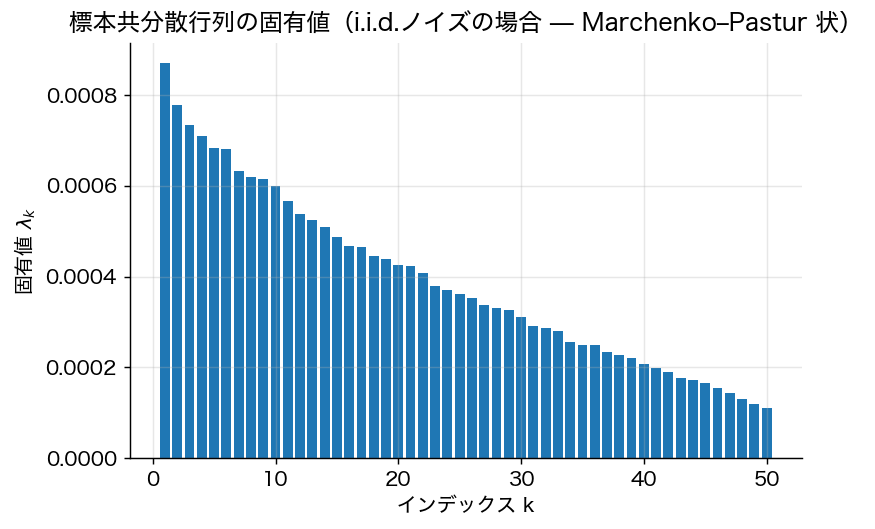
\includegraphics[width=0.85\linewidth]{figures/eigenspectrum.png}
\caption{共分散行列の固有値スペクトル例（標本$T=200$、$n=50$、i.i.d.ノイズ）。最大固有値は集中・最小固有値は $0$ に近く、最適化はこの「小さい固有値方向」を増幅するため推定誤差問題が深刻になる。}
\end{figure}

\noindent\hrulefill

% ===== 01_markowitz_basics.md =====
\chapter{第1章 Markowitz の平均分散分析}

\begin{quote}
\emph{"Diversification is both observed and sensible; a rule of behavior which does not imply the superiority of diversification must be rejected both as a hypothesis and as a maxim."}  — H. M. Markowitz (1952)
\end{quote}

\section{1.1 問題設定}

投資家が $n$ 個の危険資産に資金を配分する。リターン $R$ について $\mu = \mathbb{E}[R]$, $\Sigma = \mathrm{Cov}(R) \succ 0$ を所与とする。ポートフォリオ $w$ の

\begin{itemize}
\item 期待リターン：$\mathbb{E}[R_w] = w^\top \mu$
\item 分散（リスク）：$\mathrm{Var}(R_w) = w^\top \Sigma w$
\end{itemize}

Markowitz の中心思想は次の二つ：

\begin{enumerate}
\item \textbf{「リスク」を分散で測る}。リターンの確率分布は平均と分散の二つの値だけで（投資家にとって）十分である。
\item \textbf{平均と分散のトレードオフを明示的に最適化する}。これにより「分散投資の価値」が定量化される。
\end{enumerate}

\section{1.2 平均分散効率性}

\textbf{定義 1.1}（平均分散効率的ポートフォリオ） ポートフォリオ $w^\star$ が \textbf{効率的（efficient）} であるとは、これと同じか高い期待リターンを持ち、かつ厳密に小さい分散を持つ別のポートフォリオが存在しないことをいう。すなわち以下の問題の解として特徴付けられる：

\[ \min_{w \in \mathbb{R}^n} \tfrac{1}{2} w^\top \Sigma w \quad \text{s.t.}\quad w^\top \mu = \mu_P,\ \mathbf{1}^\top w = 1. \tag{P} \]

\section{1.3 効率的ポートフォリオの陽な表現}

問題 (P) は第0章の二次計画の枠組みに当てはまる。$A = \begin{pmatrix} \mu^\top \\ \mathbf{1}^\top \end{pmatrix}$, $b = \begin{pmatrix} \mu_P \\ 1 \end{pmatrix}$ とおき、次の \textbf{基本スカラー量} を定義する：

\[ A_0 := \mathbf{1}^\top \Sigma^{-1} \mathbf{1}, \qquad B_0 := \mathbf{1}^\top \Sigma^{-1} \mu, \qquad C_0 := \mu^\top \Sigma^{-1} \mu, \qquad D_0 := A_0 C_0 - B_0^2. \]

\textbf{補題 1.2} $\mu$ が $\mathbf{1}$ と平行でない（つまり全資産の期待リターンが同一でない）とき $D_0 > 0$。

\emph{証明方針}：$\Sigma^{-1} \succ 0$ より $(x, y) \mapsto x^\top \Sigma^{-1} y$ は内積、コーシー・シュワルツより $B_0^2 = (\mathbf{1}^\top \Sigma^{-1} \mu)^2 \le A_0 C_0$。等号は $\mu \parallel \mathbf{1}$ のときのみ。$\square$

\textbf{定理 1.3}（効率的ポートフォリオの陽な解） 問題 (P) の最適解は \[ \boxed{\; w^\star(\mu_P) = \frac{C_0 - B_0 \mu_P}{D_0}\, \Sigma^{-1} \mathbf{1} + \frac{A_0 \mu_P - B_0}{D_0}\, \Sigma^{-1} \mu \;} \] で与えられ、対応する最小分散は \[ \sigma_P^2(\mu_P) = w^{\star\top} \Sigma w^\star = \frac{A_0 \mu_P^2 - 2 B_0 \mu_P + C_0}{D_0}. \tag{1.1} \]

\emph{証明方針}：Lagrangian $L(w, \lambda_1, \lambda_2) = \tfrac{1}{2} w^\top \Sigma w - \lambda_1 (w^\top \mu - \mu_P) - \lambda_2(\mathbf{1}^\top w - 1)$。
\begin{itemize}
\item $\partial_w L = 0 \Rightarrow w = \lambda_1 \Sigma^{-1}\mu + \lambda_2 \Sigma^{-1}\mathbf{1}$。
\item 制約 $w^\top \mu = \mu_P, \mathbf{1}^\top w = 1$ に代入し $\lambda_1, \lambda_2$ について連立一次方程式を解く：
\end{itemize}
\[ \begin{pmatrix} C_0 & B_0 \\ B_0 & A_0 \end{pmatrix} \begin{pmatrix} \lambda_1 \\ \lambda_2 \end{pmatrix} = \begin{pmatrix} \mu_P \\ 1 \end{pmatrix}. \]
\begin{itemize}
\item 行列式 $D_0$ より $\lambda_1 = (A_0 \mu_P - B_0)/D_0$、$\lambda_2 = (C_0 - B_0 \mu_P)/D_0$。
\item 分散は $w^{\star\top}\Sigma w^\star = \lambda_1 \mu_P + \lambda_2$ より整理して (1.1) を得る。$\square$
\end{itemize}

\textbf{系 1.4}（大域最小分散ポートフォリオ；GMV） (1.1) を $\mu_P$ について最小化すると $\mu_P^{\rm GMV} = B_0 / A_0$、対応する重みは \[ w^{\rm GMV} = \frac{\Sigma^{-1} \mathbf{1}}{\mathbf{1}^\top \Sigma^{-1} \mathbf{1}}, \qquad \sigma_{\rm GMV}^2 = \frac{1}{A_0}. \]

\section{1.4 分散投資が機能する仕組み（直観）}

二資産の例：$\mathrm{Var}(R_w) = w_1^2 \sigma_1^2 + w_2^2 \sigma_2^2 + 2 w_1 w_2 \rho \sigma_1 \sigma_2$。相関係数 $\rho < 1$ である限り、適切な $w$ により単一資産よりリスクを低減できる。極端例として $\rho = -1$ ならば完全ヘッジが可能（リスクゼロ）。一般 $n$ 資産では、共分散行列の \textbf{小さい固有値方向} に重みを配分するほど分散が減少する。

\begin{figure}[H]
\centering
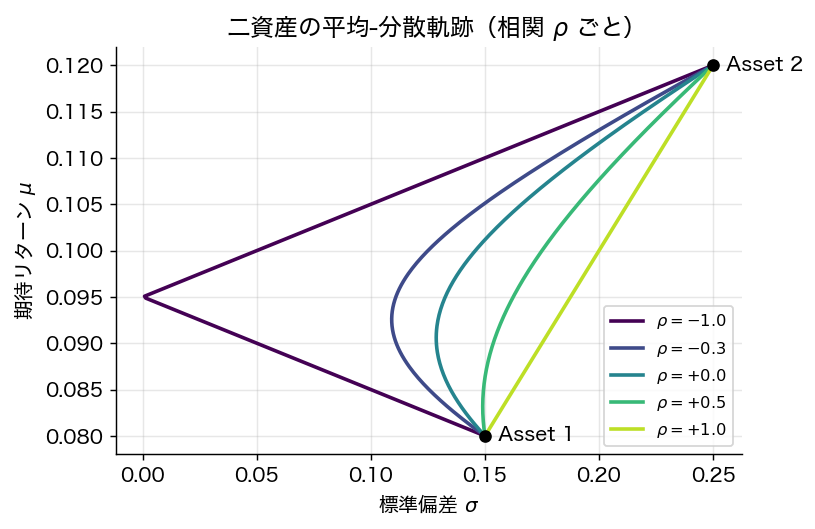
\includegraphics[width=0.85\linewidth]{figures/diversification_two_asset.png}
\caption{二資産の平均–標準偏差軌跡を相関 $\rho$ ごとに描いたもの。$\rho=-1$ ではリスクゼロのポートフォリオが構成でき、$\rho=+1$ では直線（分散投資の利益なし）。これが「分散投資のフリーランチ」の幾何的根拠。}
\end{figure}

\section{1.5 平均分散最適化の解釈}

定理 1.3 の解は \textbf{二つの基底ポートフォリオの線形結合} として書ける： \[ w^\star(\mu_P) = (1 - \alpha) w^{\rm GMV} + \alpha\, w^{\rm zero}, \] ここで $w^{\rm zero}$ は第二の基底（後章の二基金分離と直結）。これにより「効率的ポートフォリオ全体が二次元アフィン空間を成す」という鋭い構造定理が得られる。詳細は第3章。

\section{1.6 制約付き問題：ショート禁止など}

実務では $w \ge 0$ や $w_i \le \bar w_i$ などの不等式制約が課される。この場合、解は KKT 条件を満たすが \textbf{陽な閉形では書けず}、二次計画ソルバ（active set, interior point）で数値的に解く。本書では理論を見通しよく示すため、以降 $w \in \mathbb{R}^n$（ショート可）を基本とし、不等式制約は実装上の注意として扱う。

\section{1.7 推定誤差と頑健化}

実務上、$\mu, \Sigma$ は標本平均・標本共分散で推定する。Markowitz の最適化は \textbf{入力誤差を増幅する}（"error maximization" 現象）。代表的な対処：

\begin{itemize}
\item \textbf{収縮推定（shrinkage）}：Ledoit–Wolf (2004) による $\hat\Sigma$ の収縮。
\item \textbf{正則化目的関数}：$L^1$/$L^2$ ペナルティ追加（Brodie et al. 2009）。
\item \textbf{Bayes 的事前情報の取込み}：第9章の \textbf{Black–Litterman}。
\item \textbf{頑健最適化}：$\mu$ が楕円的不確実性集合に属するときの min–max。
\end{itemize}

これらは第8章・第9章で再訪する。

\section{1.8 本章のまとめ}

\begin{itemize}
\item 平均分散効率ポートフォリオは $\Sigma^{-1}\mathbf{1}$, $\Sigma^{-1}\mu$ の二つだけから合成される。
\item 最小分散は目標リターンの二次関数（双曲線、第2章で詳述）。
\item 推定誤差問題が実務上の核心的課題である。
\end{itemize}

\noindent\hrulefill

% ===== 02_efficient_frontier.md =====
\chapter{第2章 効率的フロンティアの解析的構造}

\section{2.1 フロンティアの方程式}

前章 (1.1) より $(\sigma_P, \mu_P)$ 平面において \[ \sigma_P^2 = \frac{A_0 \mu_P^2 - 2 B_0 \mu_P + C_0}{D_0} \] これは $\mu_P$ について二次なので、$(\sigma_P, \mu_P)$ 平面では \textbf{双曲線（hyperbola）} をなす。整理すると \[ \frac{\sigma_P^2}{1/A_0} - \frac{(\mu_P - B_0/A_0)^2}{D_0/A_0^2} = 1. \tag{2.1} \]

\begin{itemize}
\item \textbf{頂点}：$(\sigma, \mu) = (1/\sqrt{A_0},\ B_0/A_0)$ ＝ GMV ポートフォリオ。
\item \textbf{漸近線の傾き}：$\pm \sqrt{D_0/A_0}$。
\item \textbf{効率的フロンティア（efficient frontier）}：$\mu_P \ge B_0/A_0$ となる上半枝。
\end{itemize}

\begin{figure}[H]
\centering
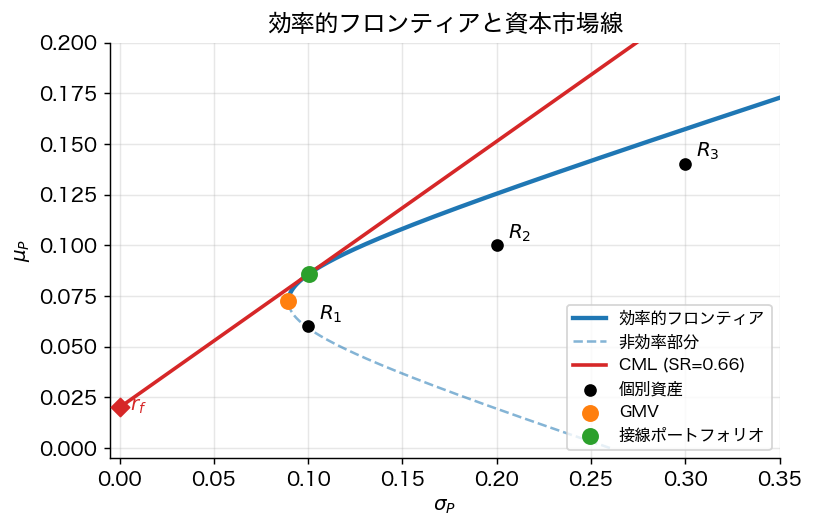
\includegraphics[width=0.85\linewidth]{figures/efficient_frontier.png}
\caption{3 資産モデルにおける効率的フロンティア（上枝の太線）、大域最小分散ポートフォリオ（GMV）、無リスク資産 $r_f$ から引いた CML、接線ポートフォリオ。CML の傾きが最大シャープ比 $\mathrm{SR}^\star$ となる。}
\end{figure}

\section{2.2 二基金分離（数学的バージョン）}

\textbf{定理 2.1} 任意の効率的ポートフォリオ $w^\star(\mu_P)$ は、\textbf{フロンティア上の任意の二つ} の異なるポートフォリオ $w^{(1)}, w^{(2)}$ の \textbf{アフィン結合} として書ける： \[ w^\star(\mu_P) = (1-t)\, w^{(1)} + t\, w^{(2)},\qquad t = \frac{\mu_P - \mu_1}{\mu_2 - \mu_1}. \]

\emph{証明方針}：定理 1.3 の解は $\mu_P$ について一次（重みが $(C_0 - B_0\mu_P)/D_0$ と $(A_0\mu_P - B_0)/D_0$）。したがって $\mu_P$ の関数として \textbf{アフィン}。二点を通るアフィン写像は唯一。$\square$

これが Tobin の \textbf{二基金分離定理} の数学的核（無リスク資産なし版）である。

\begin{figure}[H]
\centering
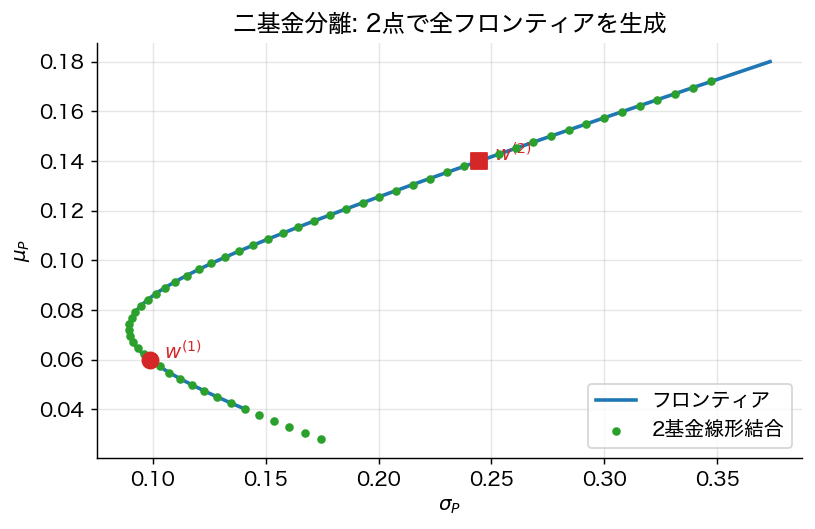
\includegraphics[width=0.85\linewidth]{figures/two_fund_separation.png}
\caption{二基金分離の幾何：フロンティア上の任意の 2 点 $w^{(1)}, w^{(2)}$ の線形結合（緑点）が完全にフロンティアの一部に一致する。「効率的ポートフォリオ全体は一次元アフィン空間」を視覚化したもの。}
\end{figure}

\section{2.3 直交分解と「ゼロ β ポートフォリオ」}

ある効率的ポートフォリオ $w_p$ に対して、\textbf{$w_p$ と無相関} な効率的ポートフォリオ $w_z$ が一意に存在し、これを $w_p$ の \textbf{ゼロ β 同伴ポートフォリオ} という。

\textbf{命題 2.2} $w_p$ の期待リターンを $\mu_p$ とするとき、ゼロ β 同伴ポートフォリオの期待リターンは \[ \mu_z(\mu_p) = \frac{C_0 - B_0 \mu_p}{B_0 - A_0 \mu_p}. \]

\emph{証明方針}：$w_z^\top \Sigma w_p = 0$ を (1.1) 周辺の代数で要求し、定理 1.3 の表現を用いて $\mu_p, \mu_z$ の関係を導く。$\square$

\textbf{幾何的意味}：$(\sigma_P, \mu_P)$ 平面において、$w_p$ における \textbf{フロンティアの接線} が縦軸（$\sigma = 0$ 軸）と交わる点が $\mu_z$。これは \textbf{Black (1972) のゼロ β CAPM} の出発点となる。

\section{2.4 接線ポートフォリオ（無リスク資産あり）}

無リスク資産（リターン $r_f$）が存在するとき、危険資産集合の効率的フロンティアからの最善は \textbf{接線ポートフォリオ} $w^T$ を介して達成される。

\textbf{定理 2.3}（接線ポートフォリオの公式） $\mu - r_f \mathbf{1} \neq 0$ かつ $\mathbf{1}^\top \Sigma^{-1}(\mu - r_f \mathbf{1}) \neq 0$ とする。シャープ比 \[ \mathrm{SR}(w) := \frac{w^\top \mu - r_f}{\sqrt{w^\top \Sigma w}} \] を最大化する $\mathbf{1}^\top w = 1$ 制約下の解は \[ \boxed{\; w^T = \frac{\Sigma^{-1}(\mu - r_f \mathbf{1})}{\mathbf{1}^\top \Sigma^{-1}(\mu - r_f \mathbf{1})} \;} \] で与えられ、最大シャープ比は \[ \mathrm{SR}^\star = \sqrt{(\mu - r_f\mathbf{1})^\top \Sigma^{-1} (\mu - r_f\mathbf{1})}. \]

\emph{証明方針}（スカラー倍同変性を活用）：シャープ比は $w$ のスケーリングに不変なので、制約 $\mathbf{1}^\top w = 1$ を外して $w^\top\Sigma w \le 1$ の下で $w^\top(\mu - r_f \mathbf{1})$ を最大化する問題と等価。Lagrangian $w^\top(\mu - r_f\mathbf{1}) - \tfrac{\lambda}{2}(w^\top \Sigma w - 1)$ より $w \propto \Sigma^{-1}(\mu - r_f\mathbf{1})$、正規化して結論。最大値はコーシー・シュワルツ型評価から $\sqrt{(\mu-r_f\mathbf{1})^\top \Sigma^{-1}(\mu-r_f\mathbf{1})}$。$\square$

\section{2.5 資本市場線（Capital Market Line; CML）}

無リスク資産と接線ポートフォリオの組合せは $(\sigma, \mu)$ 平面で \textbf{直線} をなす： \[ \mu_P = r_f + \mathrm{SR}^\star \cdot \sigma_P, \qquad \sigma_P \ge 0. \] これが \textbf{資本市場線（CML）} で、無リスク資産が利用可能な投資家の効率フロンティアとなる。すべての投資家は \textbf{「無リスク資産 + 接線ポートフォリオ」} の二点だけを組合せれば良い（Tobin の分離定理、第3章で詳説）。

\section{2.6 制約付き効率フロンティアの形}

ショート禁止 $w \ge 0$ などの不等式制約下では、効率フロンティアは \textbf{区分的に双曲線} をなす（active 制約が変わるごとに別の双曲線になる）。

\textbf{事実 2.4} 標準制約付きフロンティアは \textbf{連続かつ凹} であり、有限個の双曲線セグメントから構成される。各セグメントは「ある不等式制約の active 集合が固定された二次計画」の最適性条件を満たす。

\emph{証明方針}：パラメトリック二次計画の感度解析。$\mu_P$ の変化に対する KKT 系の連続パラメトリック解析（critical region 分析）による。$\square$

\section{2.7 数値例（コードは付録参照）}

3 資産、$r_f = 1\%$、$\mu = (8, 12, 15)^\top$\%、共分散行列を適当に与えると：
\begin{itemize}
\item GMV：分散最小、低リターン
\item 接線：シャープ比最大
\item CML：これらを結ぶ直線、危険資産の双曲線フロンティアに接する
\end{itemize}

\texttt{scripts/efficient\textbackslash{}\_frontier.py}（実装は読者の演習）で可視化できる。

\section{2.8 まとめ}

\begin{itemize}
\item 効率フロンティアは双曲線、頂点が GMV。
\item 任意の二点のアフィン結合で全フロンティアを生成（\textbf{二基金分離}）。
\item ゼロ β 同伴ポートフォリオの幾何が \textbf{Black の CAPM} の鍵。
\item 接線ポートフォリオの公式 $w^T \propto \Sigma^{-1}(\mu - r_f\mathbf{1})$ は最も実用上重要な閉形である。
\end{itemize}

\noindent\hrulefill

% ===== 03_two_fund_separation.md =====
\chapter{第3章 二基金分離定理と無リスク資産}

\section{3.1 二基金分離定理（Tobin 1958）}

\textbf{定理 3.1}（Tobin の分離定理） 無リスク資産が存在する市場において、平均分散効率的な任意のポートフォリオは \[ w_{\rm total} = (1 - \alpha) \cdot (\text{無リスク資産}) + \alpha \cdot w^T \] の形で書ける。ここで $w^T$ は危険資産だけからなる接線ポートフォリオ（第2章定理 2.3）であり、$\alpha \in \mathbb{R}$ は投資家のリスク許容度に依存する。

\emph{証明方針}：効率的問題は \[ \min_w \tfrac{1}{2} w^\top \Sigma w \quad \text{s.t.}\quad r_f + w^\top (\mu - r_f \mathbf{1}) = \mu_P \] （無リスク資産が「残り」を吸収するので $\mathbf{1}^\top w = 1$ 制約は不要）。Lagrangian $L = \tfrac{1}{2} w^\top \Sigma w - \lambda[ r_f + w^\top(\mu - r_f\mathbf{1}) - \mu_P]$ より \[ w = \lambda\, \Sigma^{-1}(\mu - r_f \mathbf{1}). \] $w$ の方向は $\mu_P$ に依存せず、スカラー $\lambda$（リスク量）のみが変化する。したがって全効率ポートフォリオは「無リスク資産 + 接線ポートフォリオの倍数」に分解される。$\square$

\textbf{経済学的含意}：投資家の選好（リスク許容度）にかかわらず \textbf{危険資産部分の構成比率は同一}。これは「市場で最適な危険資産バンドルはただ一つ」という強い主張を生み、第4章 CAPM の市場均衡論の足場となる。

\section{3.2 効用関数経由の導出}

二次効用 $u(W) = W - \tfrac{\gamma}{2} W^2$ あるいは平均分散効用 $U(w) = w^\top \mu - \tfrac{\gamma}{2} w^\top \Sigma w$ を最大化する：

\textbf{命題 3.2} $\max_w \{\,w^\top \mu - \tfrac{\gamma}{2} w^\top \Sigma w\,\}$ の解は \[ w^\star(\gamma) = \frac{1}{\gamma} \Sigma^{-1} (\mu - r_f \mathbf{1}) \] （残余は無リスク資産投資）。リスク回避度 $\gamma$ が大きいほど危険資産投資が小さい。

\emph{証明方針}：$\partial_w U = \mu - r_f\mathbf{1} - \gamma \Sigma w = 0$ より直ちに従う。$\square$

\section{3.3 効率的フロンティアの「ベクトル空間構造」}

\textbf{定理 3.3} 完全市場（$\Sigma \succ 0$、無リスク資産あり）における全ての効率ポートフォリオの集合は \textbf{二次元アフィン部分空間}（$\mathbf{1}^\top w = 1$ の下では一次元）。

\emph{証明方針}：定理 1.3 の解 $w^\star(\mu_P)$ が $\mu_P$ の一次関数であることから直ちに従う。$\square$

これは \textbf{二基金分離の数学的同値表現} である。

\section{3.4 K 基金分離}

リターン分布が \textbf{楕円的（elliptical）} な場合（多変量正規もここに含まれる）には二基金で済むが、一般のリターン分布に対して \textbf{k 基金分離} が成立する条件が知られている（Ross 1978, Cass–Stiglitz 1970）。

\textbf{事実 3.4}（Ross 1978） リターンが線形 k ファクター構造 $R = \mu + B f + \varepsilon$（$f$ は k 次元ファクター、$\varepsilon$ は特異リスク）を持つとき、効用最大化ポートフォリオは k+1 個の基金で表せる。

これは第5章の \textbf{APT} および因子モデルベースの実務（リスク予算配分）の理論的根拠を与える。

\section{3.5 無リスク資産が「短期金利」である現実}

教科書的設定では $r_f$ は確定値だが、実務では：

\begin{itemize}
\item 借入金利 > 貸出金利（\textbf{借貸金利差}）
\item 期間構造の存在（短期 vs 長期金利）
\item インフレ調整（実質金利の不確実性）
\end{itemize}

これらは効率フロンティアを \textbf{折れ線的} にし（borrow leg と lend leg で異なる接線ポートフォリオ）、純粋分離は崩れる。詳細解析は Brennan (1971) を参照。

\section{3.6 まとめ}

\begin{itemize}
\item \textbf{無リスク資産} が存在すれば全投資家は「無リスク資産 + 接線ポートフォリオ」に投資。
\item リスク許容度 $\gamma$ は \textbf{危険資産投資量} だけを決め、構成比は決めない。
\item 楕円的分布の下で完全に成立、一般には k 基金分離。
\end{itemize}

\noindent\hrulefill

% ===== 04_capm.md =====
\chapter{第4章 資本資産価格モデル（CAPM）}

Markowitz は \textbf{個人の最適化問題} を解いた。Sharpe (1964), Lintner (1965), Mossin (1966) は「全員が Markowitz 流に最適化している市場の \textbf{均衡}」が何を意味するかを問い、CAPM を導いた。

\section{4.1 均衡の仮定}

\begin{enumerate}
\item すべての投資家は同一の信念 $(\mu, \Sigma)$ を持つ（\textbf{等質期待}）。
\item すべての投資家は平均分散最適化を行う（同一時点 horizon、二次効用 or 正規分布）。
\item 共通の無リスク利子率で貸借可能。
\item 市場は完全競争・摩擦無し（取引費用・税金なし）。
\item 全資産が市場で取引される。
\end{enumerate}

仮定 1–3 より、第3章の二基金分離が \textbf{全投資家} に同時に成立する：彼らは皆 \textbf{同一の接線ポートフォリオ} $w^T$ を保有する。市場全体での保有を集計すると、$w^T$ は \textbf{市場ポートフォリオ} $w^M$（時価総額比例ウェイト）と一致せねばならない。

\section{4.2 CAPM の本体}

\textbf{定理 4.1}（CAPM、Sharpe–Lintner） 均衡において、任意の資産 $i$ のリスクプレミアムは \[ \boxed{\; \mathbb{E}[R_i] - r_f = \beta_i \cdot \big(\mathbb{E}[R_M] - r_f\big),\qquad \beta_i := \frac{\mathrm{Cov}(R_i, R_M)}{\mathrm{Var}(R_M)} \;} \] で与えられる。これを \textbf{証券市場線（Security Market Line; SML）} と呼ぶ。

\emph{証明方針 1（接線ポートフォリオ＝市場ポートフォリオ）}：
\begin{itemize}
\item 市場均衡で接線ポートフォリオが市場ポートフォリオに等しい：$w^T = w^M$。
\item 接線ポートフォリオの一階条件 $\Sigma w^T \propto \mu - r_f\mathbf{1}$ より $\mu - r_f \mathbf{1} = k\, \Sigma w^M$（ある定数 $k>0$）。
\item 各成分は $\mu_i - r_f = k \cdot \mathrm{Cov}(R_i, R_M)$。
\item 両辺の市場ポートフォリオ成分（$w^{M\top}(\mu - r_f\mathbf{1}) = k \cdot \mathrm{Var}(R_M)$）から $k = (\mathbb{E}[R_M] - r_f)/\mathrm{Var}(R_M)$。
\item 代入して結論。$\square$
\end{itemize}

\emph{証明方針 2（限界貢献の議論）}：投資家が市場ポートフォリオを保有しているとき、資産 $i$ の保有比率を微小に変えると、ポートフォリオ全体の分散は $\partial \sigma_M^2 / \partial w_i = 2\, \mathrm{Cov}(R_i, R_M)$ の比例で変化する。「リスクの限界貢献」 $\mathrm{Cov}(R_i, R_M)$ あたりのリスクプレミアム（リスク価格）が市場全体で等しいことから SML を得る。$\square$

\section{4.3 β の解釈}

\begin{itemize}
\item $\beta_i > 1$：市場よりリスキー、より高い期待超過リターン。
\item $\beta_i = 1$：市場と同じ。
\item $\beta_i < 1$：ディフェンシブ。
\item $\beta_i < 0$：市場下落時に上昇する逆相関資産（プット的）。CAPM は $\mathbb{E}[R_i] < r_f$ を予測。
\end{itemize}

\textbf{重要}：$\beta$ は \textbf{個別資産の分散} $\sigma_i^2$ ではなく \textbf{市場との共分散} に依存する。「分散できる個別リスクには対価が支払われない」というのが CAPM の核心メッセージ。

\begin{figure}[H]
\centering
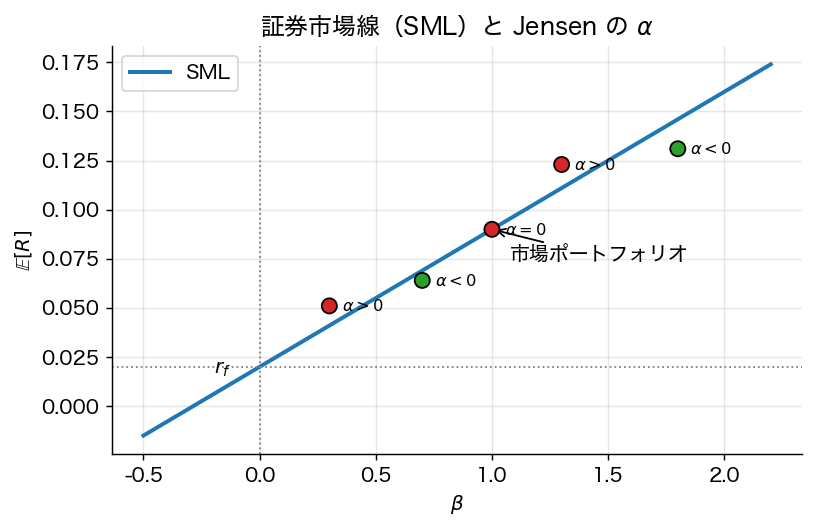
\includegraphics[width=0.85\linewidth]{figures/sml.png}
\caption{証券市場線 (SML) と Jensen の $\alpha$。SML 上にある資産は CAPM が示す均衡価格、SML より上にある資産は正の $\alpha$（割安）、下にある資産は負の $\alpha$（割高）と解釈される。}
\end{figure}

\section{4.4 Black のゼロ β CAPM}

無リスク資産が利用できない（あるいは借入金利が貸出金利と異なる）場合：

\textbf{定理 4.2}（Black 1972） 任意の効率的ポートフォリオ $w_p$ とそのゼロ β 同伴ポートフォリオ $w_z$（命題 2.2）に対して \[ \mathbb{E}[R_i] = \mathbb{E}[R_z] + \beta_i^{(p)} (\mathbb{E}[R_p] - \mathbb{E}[R_z]),\qquad \beta_i^{(p)} = \mathrm{Cov}(R_i, R_p)/\mathrm{Var}(R_p). \]

均衡では $w_p = w^M$ とすればよい。\textbf{ゼロ β 期待リターン} $\mathbb{E}[R_z]$ が $r_f$ の役割を果たす。

\emph{証明方針}：効率的フロンティア上の任意の二点の幾何（接線が縦軸と交わる切片＝ゼロ β 期待リターン）と、定理 4.1 と同じ限界貢献論証。$\square$

\section{4.5 CAPM の実証検証と Roll 批判}

代表的検証手順：\textbf{Fama–MacBeth (1973) の二段階回帰}

\begin{enumerate}
\item 時系列回帰：各資産 $i$ について $R_{it} - r_{ft} = \alpha_i + \beta_i (R_{Mt} - r_{ft}) + \varepsilon_{it}$ で $\hat\beta_i$ を推定。
\item 横断面回帰：$\bar R_i - \bar r_f = \gamma_0 + \gamma_1 \hat\beta_i + \eta_i$。CAPM が正しければ $\gamma_0 = 0$, $\gamma_1 = \bar R_M - \bar r_f$。
\end{enumerate}

実証結果：
\begin{itemize}
\item $\gamma_1 > 0$ だが $\bar R_M - \bar r_f$ より小さい（SML が \textbf{平坦}）。
\item $\gamma_0 > 0$（low β 異常）。
\item サイズ（Banz 1981）、バリュー（Fama–French 1992）などの \textbf{CAPM 残差} が説明力を持つ。
\end{itemize}

\textbf{Roll の批判（1977）}： CAPM の検証には \textbf{真の市場ポートフォリオ} $w^M$ が必要だが、これは観測不可能（全富—不動産、人的資本、海外資産—を含む）。プロキシ（株価指数）を用いた検証は実質的に「そのプロキシが平均分散効率的か」のテストにしかならない。したがって \textbf{CAPM 自体は反証不可能}。

\section{4.6 条件付き CAPM・消費 CAPM}

\begin{itemize}
\item \textbf{条件付き CAPM}：$\beta$ と市場プレミアムが時変。
\item \textbf{消費 CAPM（CCAPM, Breeden 1979, Lucas 1978）}：効用最大化の一階条件から、リスクプレミアムは \textbf{消費成長率との共分散} に比例。
\end{itemize}
\[ \mathbb{E}[R_i] - r_f = \gamma\, \mathrm{Cov}(R_i, \Delta c) \] （$\gamma$ は相対リスク回避度、$c$ は対数消費）。$M_{t+1} = \beta\, u'(c_{t+1})/u'(c_t)$ という \textbf{確率割引因子（SDF）} が中心概念となり、本書終章への橋渡しとなる。

\section{4.7 まとめ}

\begin{itemize}
\item CAPM は \textbf{「分散できないリスク（β）」だけがプレミアムを生む} ことを主張する。
\item 仮定の強さ（特に等質期待）に比して結論は強力だが、実証的には不十分。
\item Roll 批判により検証可能性自体が哲学的問題。
\item 次章の \textbf{APT} は均衡論を必要としない代替アプローチを与える。
\end{itemize}

\noindent\hrulefill

% ===== 05_apt_factor_models.md =====
\chapter{第5章 裁定価格理論（APT）とファクターモデル}

CAPM が「市場全体の効率性」という強い均衡条件を要求するのに対して、APT (Ross 1976) は \textbf{「裁定機会の不在」} という極めて弱い条件のみから多因子資産価格モデルを導出する。

\section{5.1 線形 K ファクターモデル}

各資産のリターンが \[ R_i = \mu_i + \sum_{k=1}^K b_{ik} f_k + \varepsilon_i, \qquad \mathbb{E}[f_k] = 0,\ \mathbb{E}[\varepsilon_i] = 0,\ \mathrm{Cov}(f_k, \varepsilon_i) = 0 \] で表されると仮定する。$f = (f_1, \dots, f_K)^\top$ を \textbf{共通因子（systematic factors）}、$b_i = (b_{i1}, \dots, b_{iK})^\top$ を \textbf{因子負荷量（factor loadings）}、$\varepsilon_i$ を \textbf{固有リスク（idiosyncratic risk）} という。さらに固有リスクは \textbf{資産間で無相関} とする：$\mathrm{Cov}(\varepsilon_i, \varepsilon_j) = 0\ (i \neq j)$。

行列形式：$R = \mu + B f + \varepsilon$。

\section{5.2 APT の主張と証明方針}

\textbf{定理 5.1}（APT、Ross 1976） 資産数 $n$ が十分大きく上記モデルが成立するとき、無裁定の必要条件として \[ \boxed{\; \mu_i \approx \lambda_0 + \sum_{k=1}^K b_{ik} \lambda_k\ \text{（全 } i \text{ に対して）} \;} \] が成立する。すなわち期待リターンは因子負荷量の \textbf{線形関数} で表される。$\lambda_0$ はリスクフリーレート（あるいはゼロ β 期待リターン）、$\lambda_k$ は \textbf{因子 $k$ のリスクプレミアム}。

\textbf{証明スケッチ}（裁定論証による）：

\begin{enumerate}
\item \textbf{裁定ポートフォリオの構築}：投資ゼロ（$\mathbf{1}^\top w = 0$）、因子曝露ゼロ（$B^\top w = 0$）の重み $w$ を選ぶ。
\item このポートフォリオのリターンは $w^\top R = w^\top \mu + w^\top \varepsilon$、平均は $w^\top \mu$、分散は $w^\top D w$（$D = \mathrm{diag}(\sigma_{\varepsilon_i}^2)$）。
\item $n \to \infty$ で \textbf{十分に分散} された $w$ を取れる場合、$w^\top D w \to 0$（大数の法則）。すると裁定ポートフォリオは \textbf{ほぼ確実な定数リターン} $w^\top \mu$ を持つ。
\item 無裁定条件はこれが $0$ であることを要求：$\mathbf{1}^\top w = 0$, $B^\top w = 0 \Rightarrow w^\top \mu = 0$。
\item すなわち $\mu$ は $\mathbf{1}$ と $B$ の列空間に属する：$\mu = \lambda_0 \mathbf{1} + B \lambda$。$\square$
\end{enumerate}

厳密には $n \to \infty$ の漸近的議論、誤差項 $\|\mu - \lambda_0\mathbf{1} - B\lambda\|^2$ が有界という形での主張になる。完全に厳密な定式化は Huberman (1982), Ingersoll (1984) を参照。

\section{5.3 CAPM との関係}

CAPM は \textbf{1 ファクター APT} の特別形：$K = 1$, $f_1 = R_M - \mathbb{E}[R_M]$, $b_{i1} = \beta_i$, $\lambda_0 = r_f$, $\lambda_1 = \mathbb{E}[R_M] - r_f$。

しかし APT は

\begin{itemize}
\item \textbf{市場ポートフォリオ} を明示的に必要としない（Roll 批判を回避）。
\item \textbf{均衡論} を仮定せず、無裁定のみを使う。
\item 多因子（複数の系統的リスク源）を許容する。
\end{itemize}

代償として \textbf{どの因子か} は理論的には決まらず、\textbf{経験的に選定} する必要がある。

\section{5.4 実証的ファクターモデル}

\subsection{5.4.1 Fama–French 3 ファクターモデル}

\[ R_i - r_f = \alpha_i + b_i (R_M - r_f) + s_i \cdot \mathrm{SMB} + h_i \cdot \mathrm{HML} + \varepsilon_i \]
\begin{itemize}
\item \textbf{SMB}（Small Minus Big）：小型株−大型株の超過リターン
\item \textbf{HML}（High Minus Low）：高 B/M 株−低 B/M 株（バリュー）の超過リターン
\end{itemize}

3 ファクターで CAPM の主要なアノマリ（サイズ効果、バリュー効果）を吸収。

\subsection{5.4.2 Carhart 4 ファクター}

3 ファクター + \textbf{MOM}（モメンタム：過去 12 ヶ月のリターン上位−下位）。

\subsection{5.4.3 Fama–French 5 ファクター}

3 ファクター + \textbf{RMW}（収益性）+ \textbf{CMA}（投資保守度）。

\subsection{5.4.4 Q ファクター・行動ファクター}

Hou–Xue–Zhang (2015) の Q ファクター、その他多数の「動物園（factor zoo）」。Cochrane (2011) の有名な指摘：\textbf{「ファクターの動物園」問題}。

\section{5.5 推定とリスク予算}

ファクターモデルの大きな実用利点：

\begin{itemize}
\item \textbf{共分散行列の縮約}：$\Sigma = B \Omega B^\top + D$（$\Omega$ は因子共分散、$D$ は対角の特異分散）。$n$ 資産で $n(n+1)/2$ パラメタが $nK + K(K+1)/2 + n$ に減る。\textbf{ノイズが減り、最適化が安定} する。
\item \textbf{リスク要因分解（risk attribution）}：ポートフォリオの分散を「市場リスク・スタイルリスク・銘柄選択リスク」に分解。
\item \textbf{リスク予算（risk budgeting）}：各要因への曝露量を制約として加えた最適化。
\end{itemize}

\begin{figure}[H]
\centering
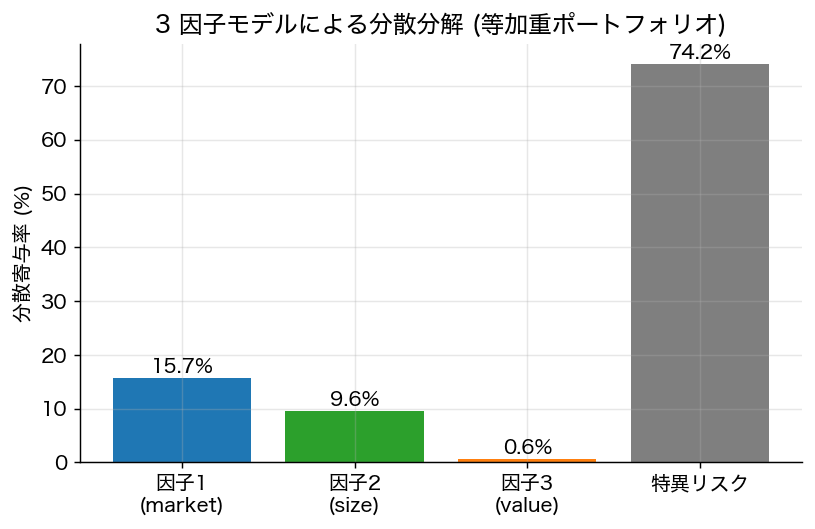
\includegraphics[width=0.85\linewidth]{figures/factor_decomposition.png}
\caption{3 因子モデル下での等加重ポートフォリオの分散寄与率分解。市場因子が支配的で、特異リスクは $n=25$ 銘柄に分散され小さい。リスクの源泉を要因別に可視化することで、運用上の意思決定（特定因子へのヘッジなど）が可能になる。}
\end{figure}

\section{5.6 主成分分析（PCA）的因子}

「観察可能なファクター」ではなく、共分散行列の \textbf{主成分} を用いる手法（\textbf{統計的因子モデル}）。Chamberlain–Rothschild (1983) の \textbf{近似因子モデル} はその理論的基礎を与え、$\Sigma$ の固有値の発散順序によって「強い因子」と「弱い因子」を区別する。

\section{5.7 まとめ}

\begin{itemize}
\item APT は \textbf{無裁定 + 大数の法則} から多因子線形価格モデルを導く。
\item CAPM の 1 因子化は厳しい仮定。実証的には 3–5 因子が支持される。
\item 因子モデルは共分散行列推定・リスク管理・パフォーマンス分析の中核技術。
\end{itemize}

\noindent\hrulefill

% ===== 06_utility_theory.md =====
\chapter{第6章 効用理論と期待効用}

平均分散分析は「リターンの平均と分散だけが効用に影響する」という強い前提に立つ。一般的にこれが正当化されるのは

\begin{itemize}
\item 投資家の効用関数が \textbf{二次} であるか、
\item リターン分布が \textbf{楕円的} であるか、
\end{itemize}

のどちらかのときだけである。本章ではより一般の期待効用理論を概観する。

\section{6.1 von Neumann–Morgenstern の公理}

確率くじ（lottery）$L \in \mathcal{L}$ 上の選好関係 $\succeq$ に対し、次の四公理：

\begin{enumerate}
\item \textbf{完備性（completeness）}
\item \textbf{推移性（transitivity）}
\item \textbf{連続性（continuity）}
\item \textbf{独立性（independence）}：$L_1 \succeq L_2 \Rightarrow \alpha L_1 + (1-\alpha) L_3 \succeq \alpha L_2 + (1-\alpha) L_3$。
\end{enumerate}

\textbf{定理 6.1}（vNM 期待効用表現定理） 上記四公理を満たす選好関係に対し、効用関数 $u: \mathbb{R} \to \mathbb{R}$（アフィン変換を除いて一意）が存在し \[ L_1 \succeq L_2 \iff \mathbb{E}_{L_1}[u(X)] \ge \mathbb{E}_{L_2}[u(X)]. \]

\emph{証明方針}：標準的くじ $\{p \cdot \bar W + (1-p) \cdot \underline W\}$ を参照基準とし、独立性公理を用いて任意のくじを「ある $p$ の標準くじと等価」と見なせる（無差別変換）。この $p$ が効用 $u(X)$ の正当な候補となる。連続性で滑らかさを担保。$\square$

\section{6.2 リスク回避}

\textbf{定義 6.2}
\begin{itemize}
\item 投資家が \textbf{リスク回避的} $\iff$ 任意の非退化くじ $X$ に対し $u(\mathbb{E}[X]) \ge \mathbb{E}[u(X)]$。
\item これは Jensen の不等式より $u$ が \textbf{凹} であることと同値。
\end{itemize}

!\href{figures/jensen\_inequality.png}{Jensen の不等式の視覚化：凹な効用 $u$ の下で、くじ $\{W_1, W_2\}$ の期待効用 $\mathbb{E}[u(W)]$（弦の中点）は確実な期待値 $\mathbb{E}[W]$ の効用 $u(\mathbb{E}[W])$（曲線上の点）より下にある。リスク回避と凹性の同値性が幾何的に見える。}

\textbf{定義 6.3}（Arrow–Pratt のリスク回避度）
\begin{itemize}
\item \textbf{絶対リスク回避度（ARA）}：$A(W) := -u''(W) / u'(W)$。
\item \textbf{相対リスク回避度（RRA）}：$R(W) := -W u''(W) / u'(W)$。
\end{itemize}

\textbf{直観}：危険資産への投資量 $\alpha^\star$ を二次近似で展開すると（小リスク近似） \[ \alpha^\star \approx \frac{\mathbb{E}[R - r_f]}{A(W)\, \sigma_R^2}. \]

\section{6.3 標準効用関数}

\begin{center}
\begin{tabular}{|l|l|l|l|}
\hline
効用 & 関数形 & ARA & RRA \\ \hline
指数（CARA） & $-e^{-\gamma W}/\gamma$ & $\gamma$（一定） & $\gamma W$ \\ \hline
べき（CRRA） & $W^{1-\gamma}/(1-\gamma)$, $\gamma\neq 1$ & $\gamma/W$ & $\gamma$（一定） \\ \hline
対数 & $\log W$ & $1/W$ & $1$ \\ \hline
二次 & $W - \tfrac{\gamma}{2}W^2$ & $\gamma/(1-\gamma W)$ & 増加 \\ \hline
\end{tabular}
\end{center}

\textbf{CARA（指数）効用} は富水準に依存せず投資量が一定。\textbf{CRRA（べき・対数）} は富比例で投資する（\textbf{実証的に支持}）。二次効用は飽和（$W > 1/\gamma$ で逆転）するため理論的に都合悪い。

\begin{figure}[H]
\centering
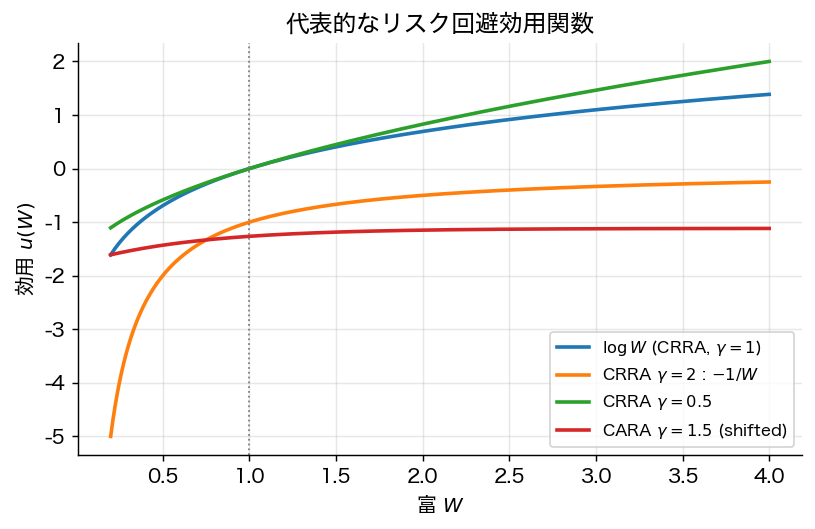
\includegraphics[width=0.85\linewidth]{figures/utility_functions.png}
\caption{代表的なリスク回避効用関数の比較。CRRA $\gamma=2$ は曲率が大きく、$\gamma$ が小さいほど線形に近づく（リスク中立に近い）。すべて凹関数だが、曲率の差がリスク回避度の差を生む。}
\end{figure}

\section{6.4 平均分散効用と期待効用の整合性}

\textbf{命題 6.4} リターンが \textbf{多変量正規分布} に従い、効用が CARA 型 $u(W) = -e^{-\gamma W}$ であるとき、期待効用最大化は \textbf{平均分散最適化} と完全に等価： \[ \max_w \mathbb{E}[u(W_0 + w^\top R)] \iff \max_w \left\{ w^\top \mu - \tfrac{\gamma W_0}{2}\, w^\top \Sigma w\right\}. \]

\emph{証明方針}：$X \sim \mathcal{N}(m, s^2)$ のとき積率母関数 $\mathbb{E}[e^{-\gamma X}] = \exp(-\gamma m + \gamma^2 s^2/2)$ を用いる。$\square$

これが Markowitz 理論の理論的正当化の核心。\textbf{正規分布の仮定が崩れる}（重尾、歪み、ジャンプ）と平均分散は近似でしかなくなる。

\section{6.5 高次モーメントの取り込み}

3 次（歪度）・4 次（尖度）モーメントを考慮した効用展開： \[ \mathbb{E}[u(W)] \approx u(\bar W) + \tfrac{1}{2} u''\sigma^2 + \tfrac{1}{6} u'''\, \mu_3 + \tfrac{1}{24} u''''\, \mu_4 + \cdots \]

$u''' > 0$（"prudence"）は \textbf{正の歪度を好む}、$u'''' < 0$（"temperance"）は \textbf{大きな尖度を嫌う}。実証的に投資家はそうした選好を示し、宝くじ的（プラス歪度）資産が「高すぎる」価格を持つ現象を生む。

\section{6.6 行動経済学的代替}

vNM 期待効用は \textbf{Allais のパラドックス} 等で実験的に反証される。代替モデル：

\begin{itemize}
\item \textbf{プロスペクト理論}（Kahneman–Tversky 1979）：参照点依存、損失回避（loss aversion）、確率歪曲関数。
\item \textbf{累積プロスペクト理論}（1992）：確率歪曲を累積分布関数に作用させる。
\item \textbf{ランク依存効用}（Quiggin 1982）。
\end{itemize}

これらは「ボラティリティ・スマイル」「モメンタム」など金融市場アノマリの説明候補となる。

\section{6.7 まとめ}

\begin{itemize}
\item 期待効用最大化は vNM 四公理から導かれる。
\item リスク回避は効用の凹性、ARA/RRA で定量化。
\item 平均分散 = 期待効用 となるのは正規分布 + CARA / 二次効用のとき。
\item 実際にはより一般の効用（CRRA、行動）と分布（非正規）が必要。
\end{itemize}

\noindent\hrulefill

% ===== 07_stochastic_dominance.md =====
\chapter{第7章 確率支配}

平均分散だけでは捉えきれない「選好」のうち、ほぼ全ての合理的投資家が同意する \textbf{頑健な順序付け} が確率支配である。

\section{7.1 一次確率支配（First-order Stochastic Dominance; FSD）}

\textbf{定義 7.1} 確率変数 $X, Y$ について $X \succeq_{\rm FSD} Y$ とは、$F_X(t) \le F_Y(t)$ がすべての $t$ で成立すること。すなわち $X$ の累積分布関数が $Y$ より「下にある」。

\textbf{定理 7.2} $X \succeq_{\rm FSD} Y \iff \mathbb{E}[u(X)] \ge \mathbb{E}[u(Y)]$ がすべての \textbf{単調非減少関数} $u$ に対して成立。

\emph{証明方針}：
\begin{itemize}
\item ($\Leftarrow$) $u(t) = \mathbf{1}_{t > s}$ という指示関数（極限的に単調）を取ると $\mathbb{E}[u(X)] = 1 - F_X(s)$、これが全 $s$ で $\ge 1 - F_Y(s)$。
\item ($\Rightarrow$) $u$ が単調非減少なら $u(t) = \int \mathbf{1}_{t > s} \mu(ds)$（Stieltjes 積分表示）で書け、各 indicator で成立する不等式を線形結合。$\square$
\end{itemize}

すなわち FSD は「より多くを好む」全ての投資家が同意する順序。

\section{7.2 二次確率支配（Second-order Stochastic Dominance; SSD）}

\textbf{定義 7.3} $X \succeq_{\rm SSD} Y$ とは $\int_{-\infty}^t F_X(s) ds \le \int_{-\infty}^t F_Y(s) ds$ が全 $t$ で成立すること。

\textbf{定理 7.4} $X \succeq_{\rm SSD} Y \iff \mathbb{E}[u(X)] \ge \mathbb{E}[u(Y)]$ がすべての \textbf{単調非減少凹関数} $u$ に対して成立。

\emph{証明方針}：
\begin{itemize}
\item ($\Leftarrow$) $u(t) = -(s - t)^+$（凹かつ単調非減少）に対する期待値が CDF の積分で書けることを示す（部分積分）。
\item ($\Rightarrow$) 任意の単調凹 $u$ を $-(s-t)^+$ 型関数の凸結合として近似（Riemann 和分解、Hardy–Littlewood–Pólya の補題）。$\square$
\end{itemize}

すなわち SSD は \textbf{「より多くを好み、かつリスク回避的な」全投資家} が同意する順序。

\textbf{重要な系}：$\mathbb{E}[X] = \mathbb{E}[Y]$ かつ $\mathrm{Var}(X) \le \mathrm{Var}(Y)$ でも、$X \succeq_{\rm SSD} Y$ は \textbf{一般には成立しない}（高次モーメントの効果）。逆に正規分布族の中では平均分散順序＝SSD 順序。

\begin{figure}[H]
\centering
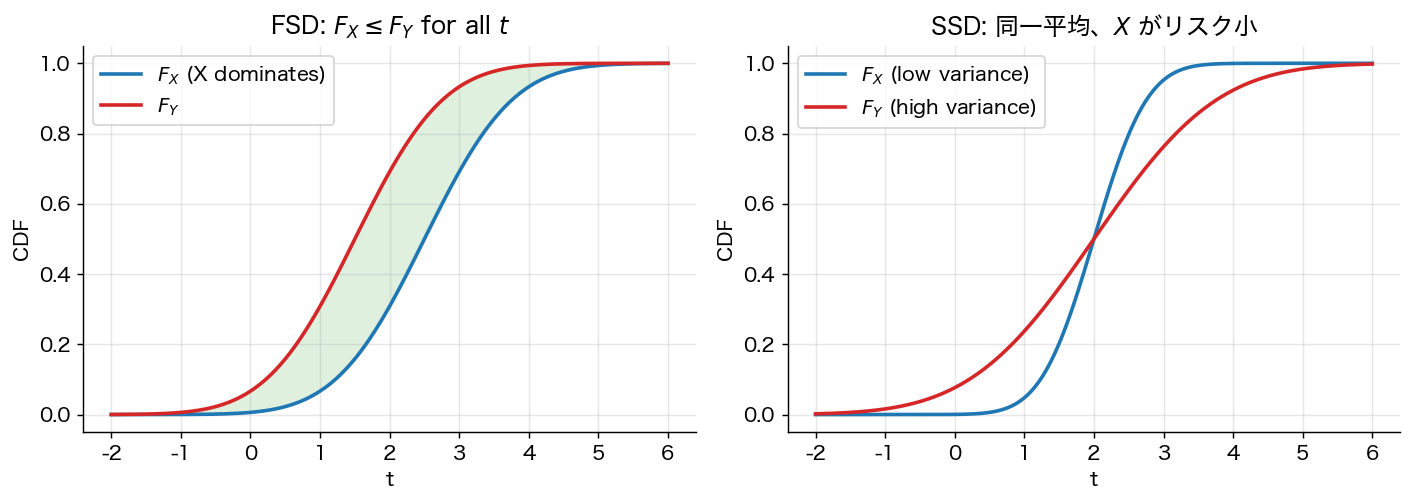
\includegraphics[width=0.85\linewidth]{figures/stochastic_dominance.png}
\caption{FSD と SSD の累積分布関数による特徴付け。左：FSD では $F_X(t) \le F_Y(t)$ が全 $t$ で成立（$X$ の CDF が常に下）。右：SSD は同じ平均で分散が小さい方が CDF 積分の意味で支配する。}
\end{figure}

\section{7.3 リスクのない/あるリスクの増大（Rothschild–Stiglitz 1970）}

\textbf{定義 7.5} $Y$ が $X$ の \textbf{平均保存スプレッド（mean-preserving spread; MPS）} であるとは、$\mathbb{E}[X] = \mathbb{E}[Y]$ かつ $Y \stackrel{d}{=} X + \varepsilon$（$\varepsilon$ は条件付き平均ゼロのノイズ）と表せること。

\textbf{定理 7.6}（Rothschild–Stiglitz） 以下は同値：
\begin{enumerate}
\item $Y$ は $X$ の MPS
\item $X \succeq_{\rm SSD} Y$（同一平均下で）
\item 全てのリスク回避効用 $u$ について $\mathbb{E}[u(X)] \ge \mathbb{E}[u(Y)]$
\end{enumerate}

\emph{証明方針}：MPS の構成性（独立ノイズ重ね合わせ）と Jensen の不等式の繰り返し適用、および「条件付き平均ゼロのノイズ追加」が Hardy–Littlewood–Pólya 型の majorization を生むこと。$\square$

\section{7.4 平均分散効率性と SSD の関係}

\textbf{事実 7.7}
\begin{itemize}
\item リターンが \textbf{多変量正規} な世界では：「平均分散効率」⇔「SSD 効率」⇔「ある CARA リスク回避者の最適化」。
\item 非正規世界では：平均分散効率は SSD 効率の \textbf{必要条件ではない}。実際、平均分散効率なポートフォリオが SSD で支配されることがある（例：ポジティブ歪度資産を排除するケース）。
\end{itemize}

これが「Markowitz 最適化が常に賢いとは限らない」具体的な根拠となる。

\section{7.5 高次の確率支配}

\textbf{$n$ 次確率支配} は順次積分した分布関数の比較で定義され、$u, u'', u^{(4)}, \dots$ の符号についての条件を満たす全ての効用に対応する。3 次以上は \textbf{慎重度（prudence）} や \textbf{節制（temperance）} といった高次性質と関連する。

\section{7.6 実用上の意義}

\begin{itemize}
\item \textbf{退職基金管理}：SSD 効率ポートフォリオを選ぶことで、加入者の効用関数を特定せずに「合理的な誰にとっても劣らない」運用を保証できる。
\item \textbf{オプション戦略}：プレミアム支払い・限定上限の戦略は平均分散では劣ることがあっても SSD では支配する/されない複雑な構造を持つ。
\end{itemize}

\section{7.7 まとめ}

\begin{itemize}
\item FSD：単調効用全体に対する順序（ほぼ普遍的）。
\item SSD：単調凹効用全体に対する順序（リスク回避者全員）。
\item MPS と SSD は同値（Rothschild–Stiglitz）。
\item 平均分散効率 ≠ SSD 効率（非正規分布下）。
\end{itemize}

\noindent\hrulefill

% ===== 08_risk_measures.md =====
\chapter{第8章 リスク尺度}

\section{8.1 リスク尺度とは何か}

リスク尺度 $\rho$ は損失分布 $L$ に実数 $\rho(L)$ を対応させる写像。標準偏差はその一例だが、

\begin{itemize}
\item 損失の \textbf{左裾（テールリスク）} に十分敏感でない
\item 対称な指標であり「損益の非対称性」を捉えない
\item 規制目的では \textbf{必要資本量} の解釈が直接できない
\end{itemize}

これらの欠点を補うのが本章のテーマである。

\section{8.2 Value-at-Risk (VaR)}

\textbf{定義 8.1} 損失 $L$ の信頼水準 $\alpha \in (0, 1)$ における VaR は \[ \mathrm{VaR}_\alpha(L) := \inf\{ x \in \mathbb{R} : P(L > x) \le 1 - \alpha\} = F_L^{-1}(\alpha) \] 通常 $\alpha = 0.95$ や $0.99$。

\textbf{バーゼル規制等で長年標準だった}。しかし以下の欠点を持つ。

\begin{figure}[H]
\centering
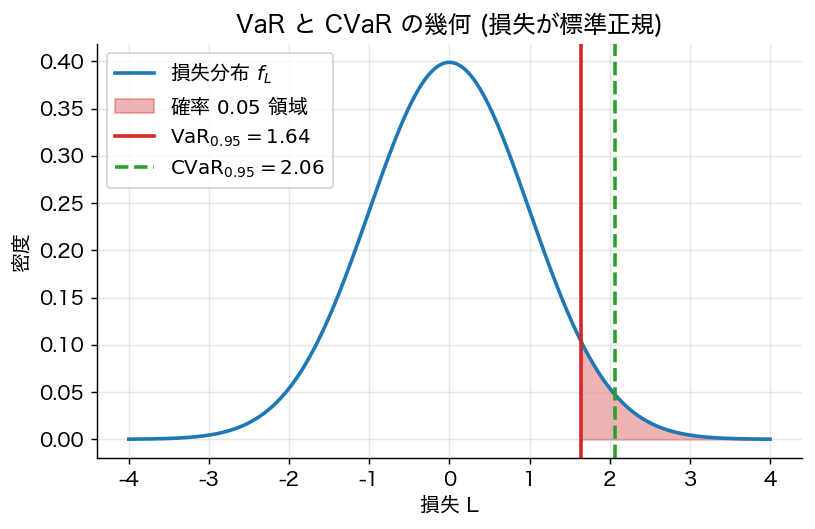
\includegraphics[width=0.85\linewidth]{figures/var_cvar.png}
\caption{VaR と CVaR の幾何的意味（損失が標準正規の場合）。VaR は分位点で「テールの境界」だけを見るのに対し、CVaR は分位点を超えた領域の \textbf{平均} を取るため、テール形状の情報を保持する。}
\end{figure}

\section{8.3 VaR の問題点：非劣加法性}

\textbf{事実 8.2} VaR は一般に \textbf{劣加法性}（$\rho(L_1 + L_2) \le \rho(L_1) + \rho(L_2)$）を満たさない。すなわち分散投資により VaR が悪化することがある。

\textbf{反例}：独立同分布の二つのデフォルト債を考える。各々 $P(\text{損失}=100) = 0.04$、$P(0) = 0.96$。$\alpha = 0.95$ で個別 VaR はいずれも 0。しかし合算 $L_1 + L_2$ の損失分布は $P(L=200) = 0.0016$, $P(L=100) = 2 \cdot 0.04 \cdot 0.96 = 0.0768$, $P(L=0) = 0.9216$。よって $\mathrm{VaR}_{0.95}(L_1 + L_2) = 100 > 0 + 0 = \mathrm{VaR}(L_1) + \mathrm{VaR}(L_2)$。

これは「分散投資をペナルティする」異常な振る舞いで、合理的なリスク管理に反する。

\begin{figure}[H]
\centering
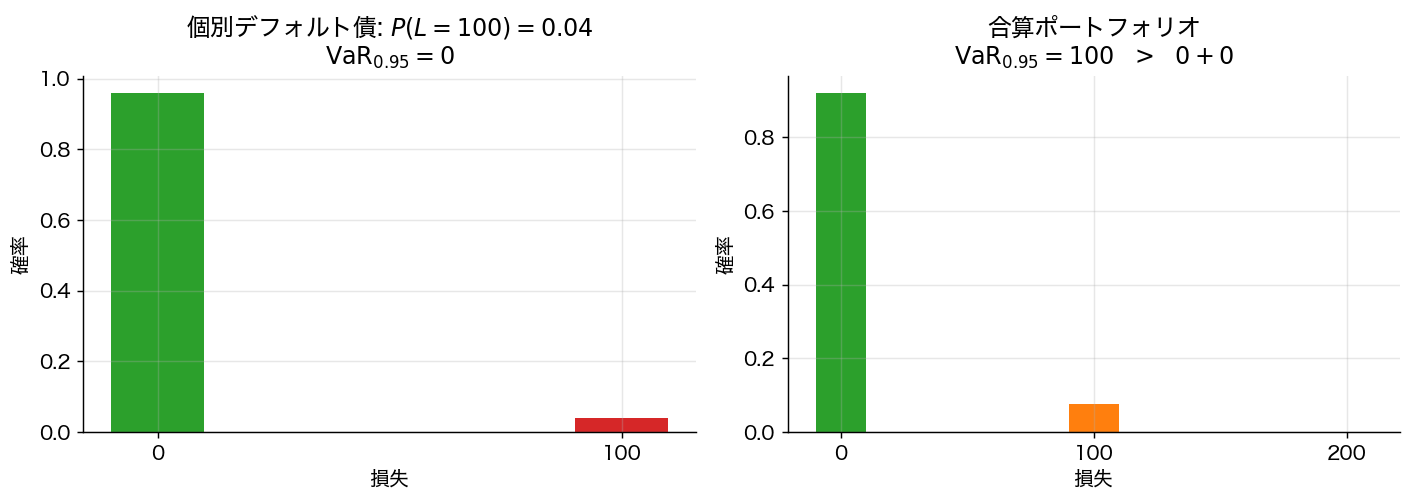
\includegraphics[width=0.85\linewidth]{figures/var_subadditivity.png}
\caption{VaR の劣加法性違反例（独立 2 デフォルト債）。左：個別の損失分布、$\mathrm{VaR}_{0.95}=0$。右：合算した分布で $\mathrm{VaR}_{0.95}=100$ となり、$0+0$ を超える。分散投資が VaR を悪化させる典型例。}
\end{figure}

\section{8.4 コヒーレントリスク尺度（Artzner et al. 1999）}

\textbf{定義 8.3}（コヒーレントリスク尺度） $\rho$ が次の四公理を満たすとき：
\begin{enumerate}
\item \textbf{単調性}：$L_1 \le L_2$ a.s. $\Rightarrow \rho(L_1) \le \rho(L_2)$
\item \textbf{平行移動不変性}：$\rho(L + c) = \rho(L) + c$（$c$ は確定損失）
\item \textbf{正同次性}：$\rho(\lambda L) = \lambda \rho(L)$（$\lambda \ge 0$）
\item \textbf{劣加法性}：$\rho(L_1 + L_2) \le \rho(L_1) + \rho(L_2)$
\end{enumerate}

\textbf{定理 8.4}（双対表現） $\rho$ がコヒーレントである必要十分条件は、ある確率測度の凸集合 $\mathcal{Q}$ が存在して \[ \rho(L) = \sup_{Q \in \mathcal{Q}} \mathbb{E}_Q[L]. \]

\emph{証明方針}：劣加法性と正同次性から $\rho$ は \textbf{凸関数（正同次凸 = 部分線形）}、Hahn–Banach の凸双対と Riesz の表現定理により、$\rho$ は確率測度の凸集合上の sup として書ける。$\square$

経済的解釈：コヒーレントリスク尺度は「最悪のシナリオ家族 $\mathcal{Q}$ における最大期待損失」。

\section{8.5 Conditional VaR / Expected Shortfall}

\textbf{定義 8.5} \[ \mathrm{CVaR}_\alpha(L) = \mathbb{E}[L \mid L \ge \mathrm{VaR}_\alpha(L)] \] （厳密には離散的分布の場合の取扱いに注意、Rockafellar–Uryasev 2000 を参照）。同義：Expected Shortfall (ES)、Tail VaR、Average VaR。

\textbf{定理 8.6} CVaR は \textbf{コヒーレント} リスク尺度。

\emph{証明方針}：双対表現 \[ \mathrm{CVaR}_\alpha(L) = \sup\bigl\{ \mathbb{E}_Q[L] : Q \ll P,\ \tfrac{dQ}{dP} \le \tfrac{1}{1-\alpha}\bigr\} \] を直接確かめ、定理 8.4 を適用。$\square$

\textbf{実務的利点}：
\begin{itemize}
\item 劣加法性のため分散投資を促進する。
\item 凸最適化と相性が良い（Rockafellar–Uryasev による線形計画化）。
\item 損失の \textbf{平均的な大きさ} を測るため、テールリスクの情報を保つ。
\end{itemize}

バーゼル III から CVaR が市場リスク資本計算の標準指標となった。

\section{8.6 CVaR 最適化（Rockafellar–Uryasev）}

\textbf{定理 8.7} ポートフォリオ $w$ の損失 $L_w(R) = -w^\top R$ の CVaR は補助関数 \[ F_\alpha(w, \zeta) := \zeta + \frac{1}{1-\alpha}\, \mathbb{E}[(L_w - \zeta)^+] \] について $\mathrm{CVaR}_\alpha(L_w) = \min_\zeta F_\alpha(w, \zeta)$。さらに $(w, \zeta)$ について同時最小化が可能で \textbf{凸最適化}（リターン分布が標本表現なら \textbf{線形計画問題}）に帰着する。

\emph{証明方針}：$\zeta = \mathrm{VaR}_\alpha$ で最小達成、これは凸関数の劣勾配法で示せる。標本表現 $R \in \{R^{(1)}, \dots, R^{(S)}\}$ では $(L_w^{(s)} - \zeta)^+ = u_s$、$u_s \ge 0$、$u_s \ge L_w^{(s)} - \zeta$ の線形緩和で書ける。$\square$

これにより、\textbf{シナリオベース CVaR 最小化} は LP ソルバで効率的に解ける。

\section{8.7 スペクトラルリスク尺度・歪曲リスク尺度}

CVaR を一般化した \textbf{スペクトラルリスク尺度}： \[ \rho_\phi(L) = \int_0^1 \phi(p) \mathrm{VaR}_p(L) \, dp \] （$\phi$ は確率密度型の重み関数）。

\textbf{事実 8.8}（Acerbi 2002） $\phi$ が \textbf{非減少} ならば $\rho_\phi$ はコヒーレント。

これにより「テールに重みを大きく置く」リスク尺度を柔軟に設計できる。

\section{8.8 凸リスク尺度}

\textbf{定義 8.9}（Föllmer–Schied 2002） 劣加法性 + 正同次性を \textbf{凸性}：$\rho(\lambda L_1 + (1-\lambda) L_2) \le \lambda\rho(L_1) + (1-\lambda)\rho(L_2)$ に弱めたものを \textbf{凸リスク尺度} と呼ぶ。これにより流動性リスクや非線形なリスク（巨大ポジションの増大効果）を扱える。

双対表現は \[ \rho(L) = \sup_{Q} \{\, \mathbb{E}_Q[L] - \alpha(Q) \,\} \] （$\alpha$ は罰金関数）。

\section{8.9 動的リスク尺度（時間整合性）}

複数期間ではリスクの \textbf{時間整合性（time consistency）} が問題となる。一般に「現在から見た 2 期間の CVaR」と「明日条件付き CVaR の現在 CVaR の合成」は一致しない。時間整合的リスク尺度は \textbf{入れ子型条件付期待値表現} を持つ。詳細は Cheridito–Delbaen–Kupper (2006), Ruszczyński (2010) を参照。

\section{8.10 まとめ}

\begin{itemize}
\item VaR は実務標準だったが劣加法性を欠き、分散投資を罰しうる。
\item CVaR は劣加法性を満たし、凸最適化で扱える。
\item Artzner 公理が「合理的なリスク尺度」を特徴付ける。
\item 双対表現はリスク尺度を「最悪シナリオ族」として理解する強力な枠組み。
\end{itemize}

\noindent\hrulefill

% ===== 09_black_litterman.md =====
\chapter{第9章 Black–Litterman モデル}

Markowitz 最適化は推定誤差を増幅する（\textbf{極端なロングショート}、\textbf{入力に対する高感度}）。Black \& Litterman (1992) は \textbf{均衡を事前情報、投資家の主観的見方を観測情報} とするベイズ枠組みで、この問題を本質的に解決した。

\section{9.1 出発点：暗黙の均衡リターン}

平均分散最適化を逆向きに使う：\textbf{現実の市場ポートフォリオ $w^M$}（時価総額比例）を「均衡における最適解」と見なし、それを生成する \textbf{暗黙の期待リターン} $\Pi$ を逆算する。

平均分散効用 $U(w) = w^\top\mu - \tfrac{\gamma}{2} w^\top \Sigma w$ の最適性条件 $w^\star = \gamma^{-1} \Sigma^{-1} (\mu - r_f\mathbf{1})$ より \[ \boxed{\; \Pi = \gamma\, \Sigma\, w^M + r_f \mathbf{1} \;} \] （\textbf{Sharpe’s implied returns} とも呼ぶ）。$\gamma$ は市場全体のリスク回避度。

\section{9.2 ベイズ的見方の取り込み}

投資家は \textbf{$K$ 本の主観的な見方（views）} を持つとする。これを線形等式 \[ P \mu = Q + \eta, \qquad \eta \sim \mathcal{N}(0, \Omega) \] で表現する。
\begin{itemize}
\item $P \in \mathbb{R}^{K\times n}$：各見方が「どの資産の組合せ」に関わるか。
\item $Q \in \mathbb{R}^K$：見方の \textbf{期待値}。
\item $\Omega \in \mathbb{R}^{K\times K}$：見方の \textbf{不確実性}（対角成分が大きいほど自信が薄い）。
\end{itemize}

\textbf{例}：
\begin{itemize}
\item 「資産 A は資産 B より 3\% 高い」→ $P$ の行は $(0, \dots, 1, \dots, -1, \dots, 0)$、$Q = 0.03$。
\item 「資産 C は絶対的に 8\% のリターンを上げる」→ $P$ の行は単位ベクトル、$Q = 0.08$。
\end{itemize}

\section{9.3 事前分布と事後分布}

\textbf{事前}：$\mu \sim \mathcal{N}(\Pi, \tau \Sigma)$。スケール $\tau$ は均衡への自信度を制御（典型的に $\tau \in [0.025, 0.05]$）。

\textbf{観測}：$P \mu \sim \mathcal{N}(Q, \Omega)$。

これらをベイズ更新する。

\textbf{定理 9.1}（Black–Litterman の事後分布） 事後分布 $\mu | \text{views}$ は正規分布で、 \[ \boxed{\; \hat\mu_{\rm BL} = \bigl[(\tau\Sigma)^{-1} + P^\top \Omega^{-1} P \bigr]^{-1}\bigl[(\tau\Sigma)^{-1} \Pi + P^\top \Omega^{-1} Q\bigr] \;} \] \[ \hat\Sigma_{\rm BL,\mu} = \bigl[(\tau\Sigma)^{-1} + P^\top \Omega^{-1} P\bigr]^{-1}. \]

\emph{証明方針}：正規 × 正規の共役事前分布更新。完全平方の項を整理すれば二次形式の精度行列が和、平均が精度加重和になる標準結果。$\square$

\textbf{等価な書き直し}（数値的により安定）： \[ \hat\mu_{\rm BL} = \Pi + \tau\Sigma P^\top (P \tau\Sigma P^\top + \Omega)^{-1} (Q - P\Pi). \]

\section{9.4 リターン分布とポートフォリオ最適化}

リターン自体の事後分布は \[ R | \text{views} \sim \mathcal{N}\bigl(\hat\mu_{\rm BL},\ \Sigma + \hat\Sigma_{\rm BL,\mu}\bigr) \] （推定不確実性を加える）。

平均分散最適化に代入して、\textbf{事後ポートフォリオ} \[ w^\star_{\rm BL} = \frac{1}{\gamma}(\Sigma + \hat\Sigma_{\rm BL,\mu})^{-1}(\hat\mu_{\rm BL} - r_f\mathbf{1}). \]

実務的には $\Sigma$ のみを使う簡略版もよく見られる。

\begin{figure}[H]
\centering
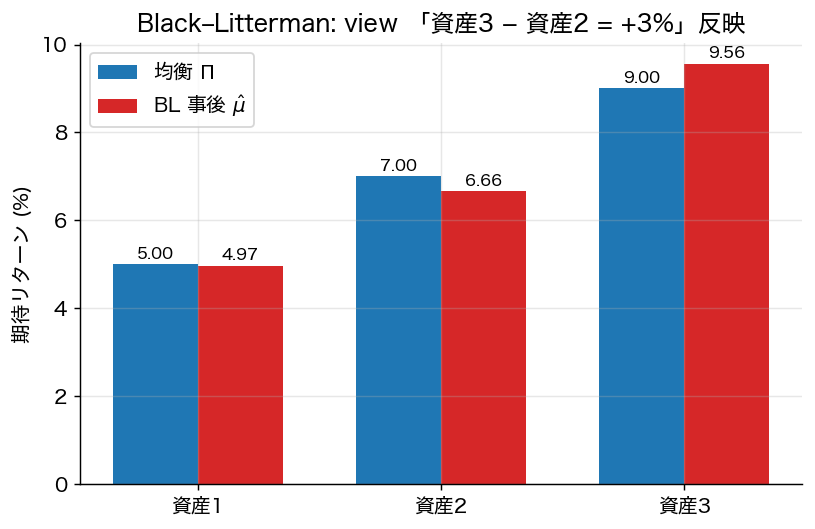
\includegraphics[width=0.85\linewidth]{figures/black_litterman.png}
\caption{Black–Litterman による期待リターンのベイズ的更新例。view「資産 3 − 資産 2 = +3\%」を反映して、資産 3 の事後リターンが上方修正され、資産 2 は下方修正される。view に関与しない資産 1 も共分散経由でわずかに更新される点に注目。}
\end{figure}

\section{9.5 Black–Litterman の魅力}

\begin{enumerate}
\item \textbf{見方を持たない資産は市場ウェイトに留まる}：$P$ にゼロを置けば、対応資産の事後は事前のまま。これにより極端な配分が抑制される。
\item \textbf{見方の自信度を $\Omega$ で連続的に調整}：$\Omega \to 0$ で見方を確信、$\Omega \to \infty$ で市場のまま。
\item \textbf{理論的に正当}：ベイズ統計の正規共役更新。
\item \textbf{実用上ロバスト}：均衡を事前にすることで「ノイズに乗っとられない」推定。
\end{enumerate}

\section{9.6 $\Omega$ の設定法}

BL 原論文は明示せず、後に複数提案：

\begin{itemize}
\item \textbf{Idzorek の方法}：各見方の「信頼度パーセンテージ」を入力すれば $\Omega$ を逆算。
\item \textbf{He–Litterman}：$\Omega = \mathrm{diag}(P \tau\Sigma P^\top)$（事前不確実性に比例）。
\item \textbf{Meucci の entropy pooling}：相対エントロピー最小化で見方を反映。
\end{itemize}

\section{9.7 例（数値例）}

3 資産（米国株、欧州株、日本株）、$\gamma = 2.5$ とする。
\begin{itemize}
\item 市場ウェイト $w^M = (0.6, 0.3, 0.1)$
\item 共分散 $\Sigma$ から $\Pi = \gamma\Sigma w^M + r_f\mathbf{1}$ を計算
\item 見方：「日本株は欧州株より 2\% 高い」→ $P = (0, -1, 1)$, $Q = 0.02$
\end{itemize}

ベイズ更新後、日本株の事後リターンが上方修正され、欧州株は下方修正。最適配分は日本株を超過配分する形になる。

\section{9.8 拡張}

\begin{itemize}
\item \textbf{Meucci のエントロピー・プーリング}：非ガウス分布、不等式型 view も扱える。
\item \textbf{Robust BL}：見方そのものに不確実性集合を許す。
\item \textbf{動的 BL}：時系列で view を更新する Kalman フィルタ的枠組み。
\end{itemize}

\section{9.9 まとめ}

\begin{itemize}
\item Black–Litterman は「均衡＝事前、view＝観測」というベイズ枠組み。
\item 推定誤差問題を本質的に緩和し、実務的に頑健なポートフォリオを生む。
\item 数式的には正規共役更新の特殊形に過ぎないが、解釈と運用性の点で革新的。
\end{itemize}

\noindent\hrulefill

% ===== 10_continuous_time_merton.md =====
\chapter{第10章 連続時間最適化：Merton 問題}

Markowitz は単期的な静的問題を扱う。実際には投資家は \textbf{時間を通じて連続的に再配分} し、しかも \textbf{消費} も行う。Merton (1969, 1971) はこの問題を確率制御として定式化し、CRRA 効用下では閉形解を得た。

\section{10.1 市場モデル}

無リスク資産：$dB_t = r B_t \, dt$

危険資産（幾何ブラウン運動）： \[ dS_t = \mu S_t \, dt + \sigma S_t \, dW_t \] （一般化して $n$ 資産：$dS_t^i / S_t^i = \mu_i \, dt + \sum_j \sigma_{ij} dW_t^j$）。

投資家は時点 $t$ に富 $X_t$ のうち $\pi_t$ の割合を危険資産に投資、$c_t$ の率で消費する。

\textbf{富の動学}（自己融資条件）： \[ dX_t = \bigl[(r + \pi_t (\mu - r)) X_t - c_t\bigr] dt + \pi_t \sigma X_t \, dW_t. \]

\section{10.2 最適化問題}

投資家は無限期間の総割引期待効用を最大化： \[ V(x) = \sup_{\pi, c} \mathbb{E}\left[\int_0^\infty e^{-\rho t} u(c_t) \, dt \;\middle|\; X_0 = x\right] \] （$\rho > 0$ は主観的割引率）。あるいは有限期間 $T$ の場合は \[ V(t, x) = \sup_{\pi, c}\mathbb{E}\left[\int_t^T e^{-\rho(s-t)} u(c_s) ds + e^{-\rho(T-t)} U(X_T)\;\middle|\; X_t = x\right]. \]

\section{10.3 動的計画原理と HJB 方程式}

\textbf{動的計画原理}： \[ V(t, x) = \sup_{\pi, c} \mathbb{E}\left[\int_t^{t+h} e^{-\rho(s-t)} u(c_s) ds + e^{-\rho h} V(t+h, X_{t+h})\;\middle|\; X_t = x\right]. \]

$h \to 0$ の極限（および $V$ の十分な滑らかさ）から、\textbf{Hamilton–Jacobi–Bellman (HJB) 方程式}：

\[ \boxed{\; 0 = \sup_{\pi, c}\Bigl\{ u(c) - \rho V + V_t + [(r + \pi(\mu - r)) x - c]\, V_x + \tfrac{1}{2} \pi^2 \sigma^2 x^2 V_{xx}\Bigr\} \;} \]

$\pi, c$ について一階条件：
\begin{itemize}
\item 消費：$u'(c) = V_x$（\textbf{包絡定理}）。
\item ポートフォリオ：$(\mu - r) x V_x + \pi \sigma^2 x^2 V_{xx} = 0$、すなわち
\end{itemize}
\[ \pi^\star = -\frac{(\mu - r) V_x}{\sigma^2 x V_{xx}}. \]

\section{10.4 CRRA 効用での閉形解}

$u(c) = c^{1-\gamma}/(1-\gamma)$（$\gamma > 0, \gamma \neq 1$）の場合、\textbf{値関数の同次性} から \[ V(t, x) = h(t) \cdot \frac{x^{1-\gamma}}{1-\gamma} \] と推測する。

\textbf{定理 10.1}（Merton 1969, 無限期間） $\rho > (1-\gamma)\bigl[r + (\mu-r)^2/(2\gamma\sigma^2)\bigr]$ の下で、最適ポートフォリオは \[ \boxed{\; \pi^\star = \frac{\mu - r}{\gamma \sigma^2} \;} \] （時間不変な定数）、最適消費は富に比例 \[ c^\star_t = m \cdot X_t,\qquad m = \frac{1}{\gamma}\left[\rho - (1-\gamma)\left(r + \frac{(\mu-r)^2}{2\gamma\sigma^2}\right)\right]. \]

\emph{証明方針}：仮定 $V = h \cdot x^{1-\gamma}/(1-\gamma)$ を HJB に代入し、$x^{1-\gamma}$ 部分を消去、$h(t)$ ないし定常解 $h$ が満たす ODE/代数方程式を解く。CRRA 同次性が「富比例」の最適消費・投資を導く。$\square$

\textbf{多資産化}：$\mu \in \mathbb{R}^n$、共分散 $\Sigma$ で $\pi^\star = \tfrac{1}{\gamma} \Sigma^{-1}(\mu - r\mathbf{1})$。これは \textbf{静的 Markowitz 接線ポートフォリオの動的版} であり、配分比率は時間不変（\textbf{myopic policy}）。

\begin{figure}[H]
\centering
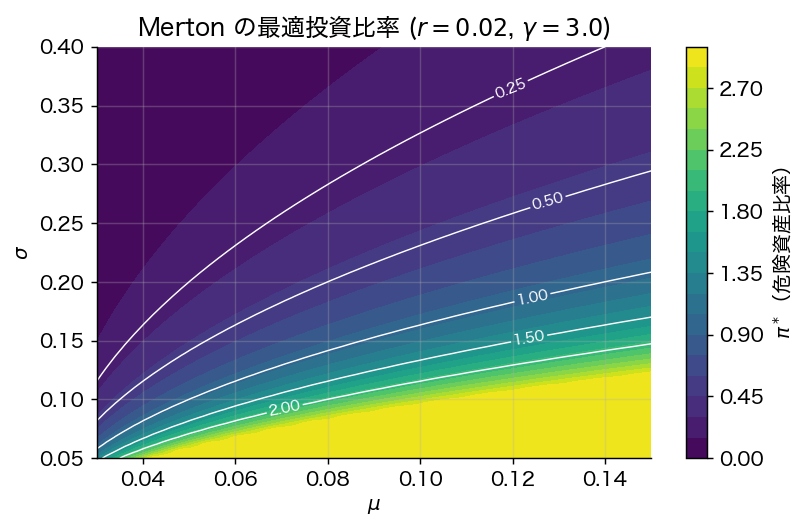
\includegraphics[width=0.85\linewidth]{figures/merton_policy.png}
\caption{Merton 問題の最適投資比率 $\pi^\star = (\mu-r)/(\gamma\sigma^2)$ を $(\mu, \sigma)$ 平面で等高線表示。ボラティリティが高いほど・期待リターンが低いほど危険資産投資を絞る。}
\end{figure}

\begin{figure}[H]
\centering
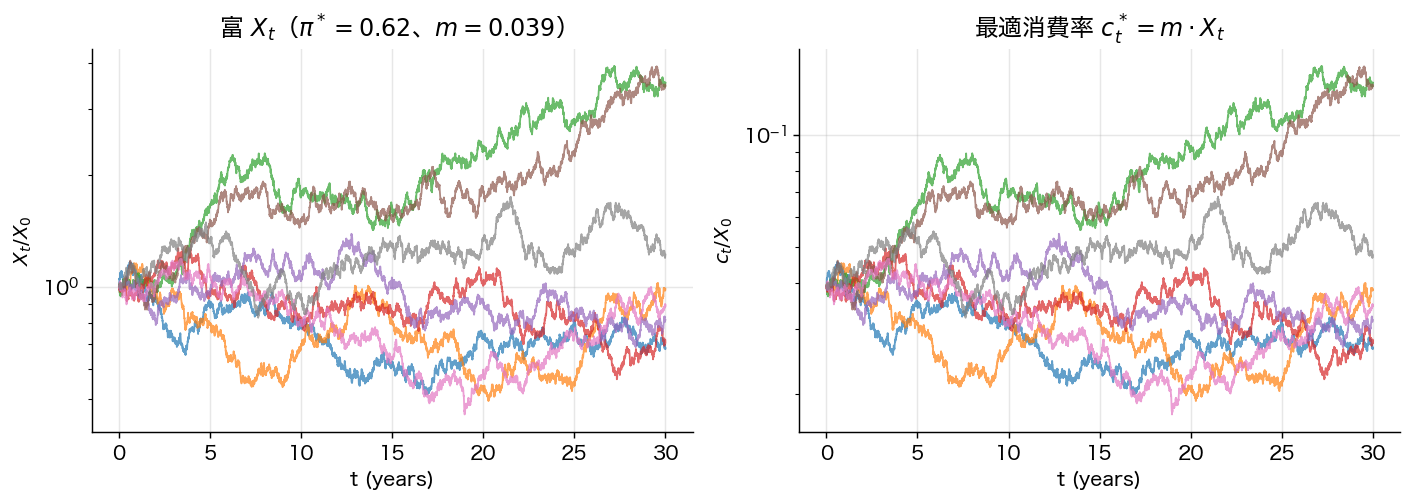
\includegraphics[width=0.85\linewidth]{figures/merton_paths.png}
\caption{Merton 問題の最適制御下での富経路と消費経路のシミュレーション（8 軌跡、$\mu=0.08, \sigma=0.18, r=0.02, \gamma=3$）。富は対数線形成長、消費は富に比例する。}
\end{figure}

\section{10.5 確率係数モデルと「ヘッジ需要」}

市場係数（$\mu, \sigma, r$）が \textbf{状態変数} $Y_t$（金利、ボラティリティ、配当利回り等）に依存し $Y_t$ が独立な確率過程に従う場合、最適投資は二項に分解：

\[ \pi^\star_t = \underbrace{\frac{\mu(Y_t) - r(Y_t)}{\gamma \sigma(Y_t)^2}}_{\text{myopic}} + \underbrace{\frac{V_{xY}}{x V_{xx}} \cdot \frac{(\rho_{SY} \sigma_Y)}{\sigma(Y_t)}}_{\text{ヘッジ需要}} \]

ヘッジ需要は \textbf{状態変動に対する効用の感度} を反映し、Merton (1973) の \textbf{異時点間 CAPM (ICAPM)} の起源となる。実証的には金利・ボラティリティのヘッジ需要が観察される。

\section{10.6 マーチンゲール法（Cox–Huang 1989, Karatzas–Lehoczky–Shreve 1987）}

完全市場では、HJB を解く代わりに \textbf{状態価格密度（state-price density）} $\xi_t$ を用い、富の動的予算制約を \textbf{単一の静的予算制約} に書き換える： \[ \mathbb{E}\left[\int_0^T \xi_t c_t \, dt + \xi_T X_T\right] \le X_0. \] ラグランジュ乗数法で \textbf{凸双対} を取り、消費と最終富を $\xi$ の関数として陽に得る。これは確率制御を \textbf{凸最適化} に帰着する強力な技法である。

\section{10.7 摩擦・制約のある拡張}

\begin{itemize}
\item \textbf{取引費用}：Davis–Norman (1990), Shreve–Soner (1994)。最適政策は「無取引帯（no-trade region）」を持つ。
\item \textbf{借入制約・空売り禁止}：自由境界問題。
\item \textbf{不完全市場}：BSDE / 二重凸双対 (Cvitanic–Karatzas)。
\item \textbf{ジャンプ過程}：Merton (1976) のジャンプ拡散モデル。
\end{itemize}

\section{10.8 連続時間 CAPM・ICAPM}

Merton (1973) は \textbf{異時点間 CAPM (ICAPM)} を提示： \[ \mathbb{E}[R_i] - r = \beta_{iM}\, (\mathbb{E}[R_M] - r) + \sum_k \beta_{ik}^Y\, \lambda_k^Y. \] 通常の市場 β に加え、\textbf{状態変数のヘッジリスクプレミアム} が現れる。これは Fama–French 等の経験的多因子モデルへの理論的橋渡しとなる。

\section{10.9 確率割引因子（SDF）と一般枠組み}

最適化の一階条件は、ある正の確率過程 $M_t$（SDF）について \[ \mathbb{E}_t[M_{t+\Delta} R_{i,t+\Delta}] = 1 \] と書ける。SDF は CCAPM（消費 CAPM、第4章末で言及）、Merton ICAPM、APT 等すべての資産価格モデルを統一する。

\section{10.10 まとめ}

\begin{itemize}
\item Merton 問題は HJB あるいはマーチンゲール法で解ける。
\item CRRA 効用下では \textbf{「Markowitz 接線比率を持ち続け、富比例で消費」} が最適。
\item 状態変数依存の係数では \textbf{ヘッジ需要} が現れ、ICAPM の多因子構造を生む。
\item 取引費用・制約・ジャンプ等の拡張は活発な研究領域。
\end{itemize}

\noindent\hrulefill

% ===== 11_performance_evaluation.md =====
\chapter{第11章 運用パフォーマンスの評価}

ポートフォリオ運用の \textbf{事後評価} は、リスク調整リターンを定量化することで「運用者は実力か運か」「ベンチマークを超えたか」を問う活動である。本章は古典的指標と統計的検出力を解説する。

\section{11.1 Sharpe 比}

\textbf{定義 11.1}（Sharpe 1966） \[ \mathrm{SR} = \frac{\mathbb{E}[R_p] - r_f}{\sigma_p}. \]

CML の傾きそのものであり、第2章定理 2.3 の最大化対象。

\textbf{統計的推定}：標本サイズ $T$、独立 i.i.d 仮定下で \[ \hat{\mathrm{SR}} - \mathrm{SR} \sim \mathcal{N}\left(0,\ \frac{1 + \mathrm{SR}^2/2}{T}\right) \quad \text{(漸近)}. \] \emph{証明方針}：デルタ法 + 標本平均・標本分散の漸近正規性。$\square$

\textbf{注意}：リターンが \textbf{正規} という仮定が標準。歪度・尖度がある場合は Sharpe 比が不適切なことがある（Mertens 2002 補正、Lo 2002）。

\begin{figure}[H]
\centering
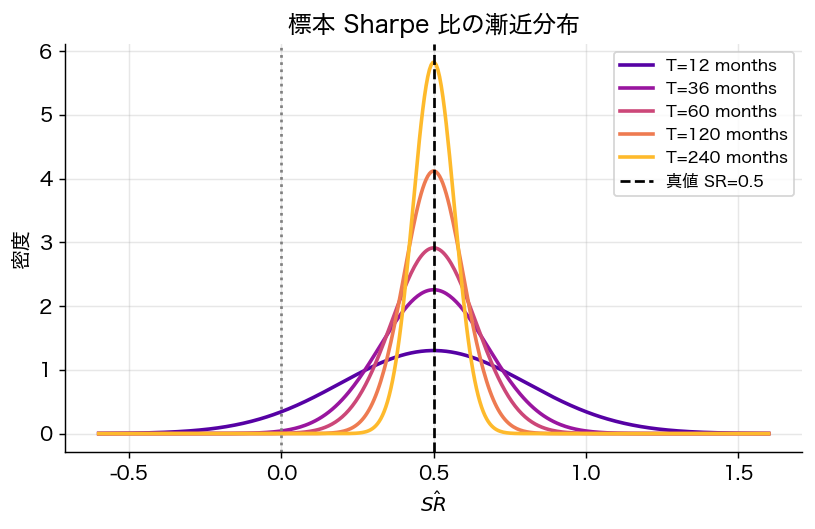
\includegraphics[width=0.85\linewidth]{figures/sharpe_distribution.png}
\caption{標本 Sharpe 比の漸近分布（真値 $\mathrm{SR}=0.5$、観測期間 $T$ ごと）。1〜3 年程度のデータでは「skill = 0」（真値ゼロ）と統計的に区別できない。長期データなしには運用者の skill を確信できないという、業界の本質的問題が見える。}
\end{figure}

\section{11.2 Treynor 比}

\[ \mathrm{Treynor} = \frac{\mathbb{E}[R_p] - r_f}{\beta_p}. \] 全分散の代わりに \textbf{β（市場リスク）} で割る。well-diversified なポートフォリオには適切だが、固有リスクが大きい場合に過大評価しがち。

\section{11.3 Jensen の α}

CAPM 回帰 \[ R_{pt} - r_{ft} = \alpha_p + \beta_p (R_{Mt} - r_{ft}) + \varepsilon_{pt} \] の切片 $\alpha_p$。CAPM が正しければ均衡で $\alpha = 0$ なので、$\alpha > 0$ は \textbf{「市場では説明できない超過リターン」}＝運用力（skill）の指標とされる。

\textbf{多因子 α}：Fama–French 3 因子回帰の切片で評価することで、サイズ・バリュー因子で説明される α を除外できる。

\section{11.4 情報比率（Information Ratio; IR）}

ベンチマーク $R_B$ に対する \textbf{アクティブリターン} $R_p - R_B$ について \[ \mathrm{IR} = \frac{\mathbb{E}[R_p - R_B]}{\mathrm{SD}(R_p - R_B)} = \frac{\alpha}{\sigma_\varepsilon}. \] \textbf{トラッキングエラー} で標準化された超過リターン。アクティブ運用の評価指標として最も重視される。

\section{11.5 Sortino 比}

下方リスクのみを罰する指標： \[ \mathrm{Sortino} = \frac{\mathbb{E}[R_p] - r_f}{\mathrm{SD}^-(R_p)}, \] ここで $\mathrm{SD}^-$ は下方半分散の平方根。投資家がアップサイドのボラを嫌わないなら理論的に Sharpe より整合的。

\section{11.6 最大ドローダウン・Calmar 比}

\textbf{最大ドローダウン}（MDD）：累積価値のピークから谷底までの最大下落率 \[ \mathrm{MDD} = \sup_{0 \le s \le t \le T} \left(1 - \frac{V_t}{V_s}\right). \] \textbf{Calmar 比} $= \mathbb{E}[R] / \mathrm{MDD}$（典型的に年率）。

\begin{figure}[H]
\centering
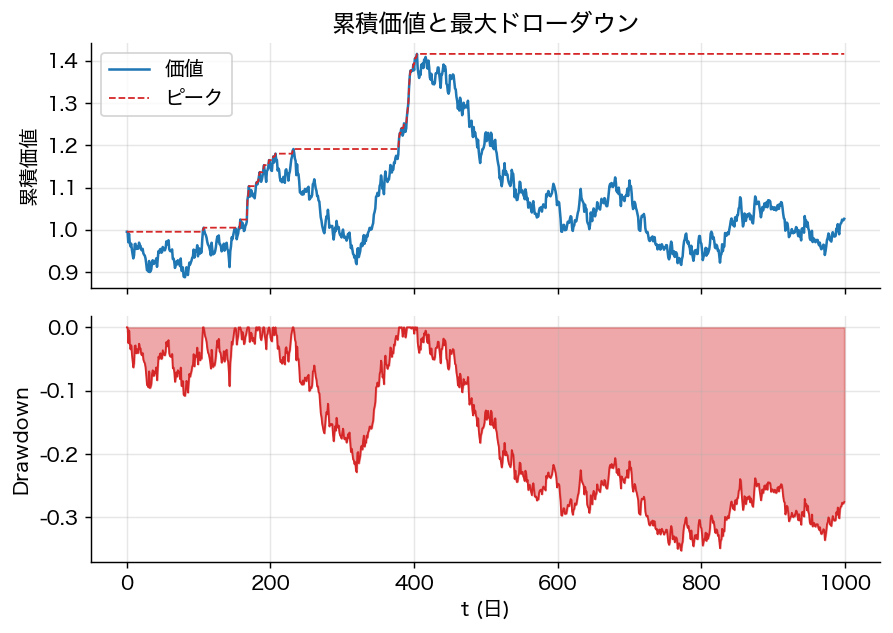
\includegraphics[width=0.85\linewidth]{figures/drawdown.png}
\caption{累積価値とドローダウンの可視化。上図：価値推移とピーク（赤破線）。下図：各時点のドローダウン。Sharpe 比だけでは現れない「投資家心理を試される深い谷」を Calmar 比で評価する。}
\end{figure}

\section{11.7 リスク調整パフォーマンスの数学的洞察}

\textbf{事実 11.2} 任意の運用戦略について、Sharpe 比は \textbf{時間にスケールする}： \[ \mathrm{SR}_{\text{年率}} = \sqrt{n} \cdot \mathrm{SR}_{\text{日次}} \] （独立同分布リターン仮定）。年率化は単純に $\sqrt{T}$ 倍。

\textbf{事実 11.3}（Bailey–López de Prado 2014） バックテストにおいて、複数の戦略から最良を選んだ「事後選択 Sharpe」は \textbf{大幅にバイアスがかかる}： \[ \mathbb{E}[\max_i \widehat{\mathrm{SR}}_i] \approx \sigma_{\mathrm{SR}} \cdot \sqrt{2\log N} \] （$N$ は戦略数）。\textbf{Deflated Sharpe Ratio} で補正が必要。

\section{11.8 検出力：必要サンプル}

「ある真の Sharpe 比が $\mathrm{SR}$ で正であるか有意性 5\%・検出力 80\% で確認するための最低期間」は概算 \[ T \gtrsim \frac{(1.96 + 0.84)^2 (1 + \mathrm{SR}^2/2)}{\mathrm{SR}^2}. \] たとえば $\mathrm{SR} = 0.5$ 年なら約 32 年必要。\textbf{多くのファンドが「実力か運か」統計的に判別不能}。

\section{11.9 リスク帰属・パフォーマンス帰属}

\begin{itemize}
\item \textbf{Brinson 分解}：超過リターンを「アロケーション効果・銘柄選択効果・相互作用効果」に分解。
\item \textbf{リスク要因帰属}：ファクターモデルで分散を要因別に分解。
\item \textbf{時系列回帰 α + 横断面回帰}：Fama–MacBeth 型評価。
\end{itemize}

\section{11.10 リスク調整指標の関係}

\begin{center}
\begin{tabular}{|l|l|l|l|}
\hline
指標 & リスク尺度 & ベンチマーク & 仮定 \\ \hline
Sharpe & 全分散 & 無リスク & 正規分布 \\ \hline
Treynor & β & 無リスク & 完全分散 \\ \hline
Jensen α & 残差分散 & CAPM & CAPM 妥当性 \\ \hline
IR & TE（残差分散） & 指数 & — \\ \hline
Sortino & 下方分散 & 目標 & 下方リスク選好 \\ \hline
\end{tabular}
\end{center}

\section{11.11 まとめ}

\begin{itemize}
\item Sharpe 比は最も普及した指標だが、正規分布・i.i.d 仮定に依存。
\item Jensen α と IR は α 検出に有用。
\item バックテスト Sharpe は \textbf{データスヌーピング} で著しくバイアス。
\item 統計的に skill を実証するには \textbf{長期データ＋多重比較補正} が必須。
\end{itemize}

\noindent\hrulefill

% ===== 12_exercises.md =====
\chapter{第12章 演習問題}

各章の理解を確認・拡張する問題集。難易度 ★（基本）/ ★★（応用）/ ★★★（発展）。

\section{第1–2章：Markowitz と効率的フロンティア}

\textbf{問題 1.1（★）} 2 資産（$\mu = (0.08, 0.12)^\top$、$\sigma_1 = 0.15$、$\sigma_2 = 0.25$、相関 $\rho = 0.3$）について、GMV ポートフォリオの重みと分散を求めよ。

\textbf{問題 1.2（★★）} $\Sigma = \sigma^2 I_n$（独立同分散）のとき、効率的フロンティアを陽に表せ。$n \to \infty$ で何が起こるか考察せよ。

\textbf{問題 1.3（★★★）} ショート禁止制約 $w \ge 0$ の下で、効率フロンティアが \textbf{区分的双曲線} であることを active set 分析で示せ。

\textbf{問題 2.1（★）} 3 資産で $r_f = 0.02$、$\mu = (0.06, 0.10, 0.14)^\top$、$\Sigma = \mathrm{diag}(0.01, 0.04, 0.09) + 0.005\, \mathbf{1}\mathbf{1}^\top$ とする。接線ポートフォリオを計算し、最大シャープ比を求めよ。

\textbf{問題 2.2（★★）} ゼロ β 同伴ポートフォリオの期待リターン公式（命題 2.2）を導出せよ。

\section{第3–4章：分離定理と CAPM}

\textbf{問題 3.1（★）} リスク回避度 $\gamma$ の二次効用について、無リスク資産と接線ポートフォリオへの配分比を求めよ。

\textbf{問題 4.1（★★）} $n$ 資産のリターンを観測した。サンプル共分散行列の固有値構造から市場ポートフォリオを推定する手順を Fama–MacBeth 二段階回帰の枠組みで述べよ。

\textbf{問題 4.2（★★★）} Roll 批判の数学的内容を述べ、観測されたプロキシポートフォリオが効率的でない場合に、CAPM 検定の null 仮説が成立しないことを示せ。

\section{第5章：APT}

\textbf{問題 5.1（★★）} 2 ファクターモデル $R_i = \mu_i + b_{i1} f_1 + b_{i2} f_2 + \varepsilon_i$ で $n \to \infty$ における裁定ポートフォリオを陽に構築し、定理 5.1 の証明を補強せよ。

\textbf{問題 5.2（★★）} Fama–French 3 因子モデルの月次データ（Kenneth French のウェブサイトから取得可能）を用いて、ある産業ポートフォリオの α を推定する Python コードを書け。

\section{第6–7章：効用理論と確率支配}

\textbf{問題 6.1（★）} CRRA 効用 $u(c) = c^{1-\gamma}/(1-\gamma)$ について ARA, RRA を計算し、$\gamma \to 1$ で対数効用になることを示せ。

\textbf{問題 6.2（★★）} リターンが対数正規分布 $\log(1 + R) \sim \mathcal{N}(m, s^2)$ のとき、CRRA 効用最大化問題を解いて最適投資比率を求めよ。

\textbf{問題 7.1（★★）} $X \sim \mathrm{Uniform}(0,1)$、$Y \sim \mathrm{Beta}(2, 2)$ について FSD/SSD 関係を判定せよ。

\textbf{問題 7.2（★★★）} 平均分散効率なポートフォリオが SSD 効率でない反例を構築せよ。

\section{第8章：リスク尺度}

\textbf{問題 8.1（★）} $L \sim \mathcal{N}(\mu, \sigma^2)$ について $\mathrm{VaR}_\alpha$ と $\mathrm{CVaR}_\alpha$ を陽に求めよ。

\textbf{問題 8.2（★★）} 8.3 節の反例（独立デフォルト債）を一般化し、VaR が劣加法性を破るパラメタ範囲を特定せよ。

\textbf{問題 8.3（★★★）} Rockafellar–Uryasev の補助関数 $F_\alpha(w, \zeta)$ が $\zeta$ について凸であり、最小値が CVaR に等しいことを証明せよ。

\section{第9章：Black–Litterman}

\textbf{問題 9.1（★★）} 3 資産で view が「資産 1 と 2 の平均は資産 3 より 3\% 高い」とするとき、$P, Q$ を書き下し、$\Omega$ を He–Litterman 法で設定する手順を示せ。

\textbf{問題 9.2（★★★）} 事後分布の式 9.4 を完全平方の整理から導出せよ。

\section{第10章：連続時間最適化}

\textbf{問題 10.1（★★）} CRRA 効用の Merton 問題で値関数 $V(t, x) = h(t) x^{1-\gamma}/(1-\gamma)$ と推測し、$h(t)$ の ODE を導け。

\textbf{問題 10.2（★★★）} 2 危険資産・確率ボラティリティ（Heston モデル）の最適投資問題で、ヘッジ需要項を陽に書き下せ。

\textbf{問題 10.3（★★★）} Cox–Huang のマーチンゲール法を用いて、CRRA 投資家の終末富と消費を陽に求めよ。

\section{第11章：パフォーマンス評価}

\textbf{問題 11.1（★）} 年率 Sharpe 比 0.8 のファンドを、5\% 有意水準で「skill > 0」と検出するに必要な最低期間（年）を概算せよ。

\textbf{問題 11.2（★★）} 独立に 1000 通りの戦略をバックテストし、最大の標本 Sharpe を選んだ。真の Sharpe がすべてゼロのとき、その期待値の概算式を示せ。

\textbf{問題 11.3（★★）} Sortino 比、Calmar 比、Sharpe 比のいずれが「ヘッジファンドのパフォーマンス比較」に最適か議論せよ。

\section{総合演習}

\textbf{問題 T.1（★★★）} S\&P 500 構成銘柄の日次リターン（過去 10 年）から共分散行列を推定し、(a) 標本共分散、(b) Ledoit–Wolf 縮約、(c) Fama–French 3 因子モデルベースで、それぞれ接線ポートフォリオを構築せよ。アウト・オブ・サンプル Sharpe を比較せよ。

\textbf{問題 T.2（★★★）} Black–Litterman ベイズフレームワークを用いて、グローバル株式・債券・コモディティの戦略的アセットアロケーションを設計せよ。市場ポートフォリオ・自身の view・$\Omega$ の選択を明示し、ポートフォリオの感度解析を行え。

\textbf{問題 T.3（★★★）} Merton 問題に税金（短期/長期キャピタルゲイン税の違い）を導入したときの最適政策を考察せよ。理論的考察と数値シミュレーションの両方を行え。

\noindent\hrulefill


\end{document}
